\documentclass[journal]{IEEEtran}
\usepackage{graphicx}
\graphicspath{{figures/}{./}}
\usepackage{amsmath}
\usepackage{amssymb}
\usepackage{cite}
\usepackage[utf8]{inputenc}
\usepackage{url}
\usepackage[T1]{fontenc}
\usepackage{xcolor}
\usepackage{tikz}
\usetikzlibrary{arrows.meta,positioning,calc,fit,backgrounds,shapes.geometric}
\usepackage{booktabs}
\usepackage{tabularx}
% search-string column: ragged right and never hyphenated, so a string pastes exactly as printed
\newcolumntype{S}{>{\raggedright\arraybackslash\hyphenpenalty=10000\exhyphenpenalty=10000}X}
\usepackage{algorithm}
\usepackage{algpseudocode}
\usepackage{listings}
%% Search strings are printed as listings, not as a table: they must stay
%% character-exact and paste-able, which table line breaking cannot guarantee.
\lstset{basicstyle=\ttfamily\scriptsize,breaklines=true,breakatwhitespace=false,
  columns=fullflexible,keepspaces=true,frame=none,xleftmargin=0pt,aboveskip=4pt,belowskip=8pt}

%% Float placement: let full-width tables share pages with body text.
\renewcommand{\topfraction}{0.92}
\renewcommand{\bottomfraction}{0.7}
\renewcommand{\textfraction}{0.06}
\renewcommand{\floatpagefraction}{0.88}
\renewcommand{\dbltopfraction}{0.92}
\renewcommand{\dblfloatpagefraction}{0.88}
\setlength{\textfloatsep}{12pt plus 2pt minus 2pt}
\setlength{\dbltextfloatsep}{12pt plus 2pt minus 2pt}
\setlength{\floatsep}{10pt plus 2pt minus 2pt}
\setlength{\dblfloatsep}{10pt plus 2pt minus 2pt}
\setcounter{topnumber}{3}
\setcounter{dbltopnumber}{3}
\setcounter{totalnumber}{5}

\begin{document}

\title{Spatiotemporal Deep Learning for IoT-Enabled Digital Health: A Survey of Model Architectures, Deployment Constraints, and Digital Twins}

\author{Xin~Xiang,~Hua~Fang,~Dengyi~Liu,~Ashikur~Nobel,~and~Honggang~Wang%
\thanks{The authors are with the Graduate Computer Science and Engineering Department, Katz School of Health and Science, Yeshiva University, New York, NY 10016 USA (e-mail: xxiang@mail.yu.edu; julia.fang@yu.edu; dliu6@mail.yu.edu; anobel@mail.yu.edu; honggang.wang@yu.edu).}}

\maketitle

\begin{abstract}
Existing surveys discuss spatiotemporal learning, Internet of Things (IoT) health systems, and digital twins from different perspectives, leaving acquisition and deployment constraints insufficiently connected to model evaluation. This focused critical survey develops an IoT-aware taxonomy that links sensing modality, sampling cadence, spatial structure, connectivity, and inference placement to candidate model families and validation requirements. A logged title-and-abstract search identified 593 records passing textual screening rules. Separately, an illustrative synthesis examines 22 purposively assembled studies: twelve retained from earlier drafting and ten selected from the PubMed screening pool. This set supports within-study comparisons and failure analysis, but does not estimate the prevalence of capabilities across the literature. We distinguish explicitly modeled spatial structure from multichannel and temporal-only inputs, and assess reported predictive results alongside split design, uncertainty, and measured resource costs. Subject-level and record-level evaluations support different deployment claims; a portable-device measurement establishes only the tested configuration. The survey translates these observations into practical guidance on resource budgeting, missing-data handling, external validation, and synchronization. It also distinguishes patient-specific prediction from a synchronized digital twin and action-conditioned simulation from identified intervention effects. The resulting framework provides a structured basis for selecting and evaluating connected-health models while keeping conceptual world-model capabilities separate from demonstrated clinical evidence.
\end{abstract}

\begin{IEEEkeywords}
Spatiotemporal models, deep neural networks, digital health, Internet of Things, wearable sensing, edge computing, federated learning, digital twin, world models.
\end{IEEEkeywords}

\section{Introduction}
\label{sec:intro}
\begin{table*}[tp]
\centering
\caption{Recent reviews adjacent to this survey, compared purposively rather than through an exhaustive search for surveys. $\bullet$ substantive coverage, $\circ$ partial coverage, -- not coded as a focus in the retained extraction. These are qualitative scope judgments, not quality scores or guarantees of absence. Samani et al.\ and Gao et al.\ are coded from their abstracts; their negative marks mean not established from that abstract. Supporting locations are in audit file A01 (Section~\ref{sec:selection}); the coding is by a single reviewer and has not been independently re-audited. IoT: IoT layer (acquisition tier); ST: spatiotemporal model families; App: clinical application; DT: digital twin; WM: world model; Priv: privacy; Edge: edge deployment; Data: datasets; Eval: evaluation.}
\label{tab:related-surveys}

\footnotesize
\setlength{\tabcolsep}{2.5pt}
\renewcommand{\arraystretch}{1.12}
\begin{tabularx}{\textwidth}{|>{\raggedright\arraybackslash}p{2.15cm}|c|c|c|c|c|c|c|c|c|>{\raggedright\arraybackslash}X|>{\raggedright\arraybackslash}p{0.95cm}|}
\hline
Review & IoT & ST & App & DT & WM & Priv & Edge & Data & Eval & Note & Ref. \\
\hline
Wang et al. & -- & $\bullet$ & $\circ$ & -- & -- & -- & -- & -- & -- & General ST mining; emphasis outside patient-specific deployment & \cite{wang2022deep} \\
\hline
Samani et al. & -- & $\bullet$ & -- & -- & -- & -- & -- & $\circ$ & -- & General prediction; abstract only & \cite{samani2026stdl} \\
\hline
Swinckels et al. & -- & $\circ$ & $\bullet$ & -- & -- & -- & -- & $\bullet$ & -- & Longitudinal EHR; no sensing tier, no critical appraisal & \cite{swinckels2024ehr} \\
\hline
Busnatu et al. & $\bullet$ & -- & $\bullet$ & -- & -- & $\circ$ & -- & -- & -- & Biotelemetry devices; no model families & \cite{Busnatu2022} \\
\hline
Sun et al. & -- & $\circ$ & $\bullet$ & -- & -- & -- & -- & $\bullet$ & $\bullet$ & Irregular medical series; temporal only & \cite{sun2026irregularmedical} \\
\hline
Wang et al. & $\bullet$ & -- & -- & $\bullet$ & -- & $\bullet$ & $\bullet$ & -- & -- & Industrial IoT twins, not patient twins & \cite{Wang2023Survey} \\
\hline
Sel et al. & -- & -- & $\circ$ & $\bullet$ & -- & $\circ$ & -- & -- & $\bullet$ & Verification, validation, and uncertainty for precision medicine & \cite{Sel2025VVUQ} \\
\hline
Zheng et al. & $\circ$ & -- & -- & $\bullet$ & $\bullet$ & $\circ$ & $\bullet$ & -- & -- & Mobile edge intelligence, not clinical care & \cite{Zheng2026DTtoWM} \\
\hline
Chen et al. & $\bullet$ & -- & $\bullet$ & $\bullet$ & -- & $\circ$ & -- & -- & -- & Generative human twins; no model comparison & \cite{chen2024genaitwin} \\
\hline
Amin \& Hossain & $\bullet$ & -- & $\bullet$ & -- & -- & $\circ$ & $\bullet$ & -- & -- & Edge-AI offloading; no model families or twins & \cite{amin2021edgeintel} \\
\hline
Nguyen et al. & $\bullet$ & -- & $\bullet$ & -- & -- & $\bullet$ & $\circ$ & -- & -- & Federated aggregation; no spatiotemporal learning & \cite{nguyen2022FLsmarthealthcare} \\
\hline
Zhang et al. & $\circ$ & $\bullet$ & $\bullet$ & -- & -- & $\circ$ & $\circ$ & $\bullet$ & -- & Wearable activity recognition; no twin layer & \cite{zhang2022harreview} \\
\hline
Gao et al. & $\bullet$ & -- & $\bullet$ & -- & -- & -- & $\bullet$ & -- & $\circ$ & Closed-loop wearable sensing and therapy; no twin or world-model layer & \cite{gao2026closedloop} \\
\hline
Wimalasiri & -- & $\circ$ & $\bullet$ & -- & $\bullet$ & -- & -- & -- & $\bullet$ & Verification framework; audit of nine imaging world models; no IoT tier & \cite{wimalasiri2026verifiable} \\
\hline
Chen et al. & -- & $\circ$ & $\bullet$ & $\circ$ & $\bullet$ & -- & -- & $\circ$ & $\bullet$ & Medical world models (preprint); no acquisition or placement layer & \cite{chen2026medicalwm} \\
\hline
This survey & $\bullet$ & $\bullet$ & $\bullet$ & $\bullet$ & $\bullet$ & $\bullet$ & $\bullet$ & $\bullet$ & $\bullet$ & IoT-aware decision map (Fig.~\ref{fig:taxonomy}, Table~\ref{tab:decision}); within-study comparison; evidence stages & -- \\
\hline
\end{tabularx}

\end{table*}

In IoT-enabled digital health, the deployed system decides what a model can learn. Wearables, continuous glucose monitors (CGM), ambient nodes and smartphones acting as gateways fix which variables exist, at what rate, with what gaps and under which timestamp and calibration conventions; the network and edge layers fix where a model may run and how fast it must respond. Temporal models can forecast future glucose measurements from CGM histories~\cite{Li2020GluNet}---and location, food environment, activity and socioeconomic context shape the same trajectories~\cite{McCullough2022Diet}, which motivates jointly examining temporal and spatial information when both are actually available to the model. What is unresolved is the design question that connects the two: given a sensing modality, a sampling cadence, a link budget and an inference placement, which model families are suitable, and what evidence must a model show before it is trusted at the edge, across federated sites, or inside a digital twin of one patient?

Table~\ref{tab:related-surveys} sets this survey against fifteen adjacent reviews and frameworks, chosen by the authors to span the five neighboring literatures---spatiotemporal modeling, longitudinal clinical modeling, IoT and edge health systems, digital twins, and world models---rather than by a systematic procedure; three appeared in 2026 and were added at this revision. The closest is a medical world-model review that maps 98 sources, finds most systems retrospective or preclinical, and warns that action-conditioned prediction is not counterfactual inference~\cite{chen2026medicalwm}; a companion framework audits nine imaging world models for fidelity, roll-out stability and clinical plausibility~\cite{wimalasiri2026verifiable}. Both start from the model. Neither asks what the sensing tier, the link and the inference placement allow a model to observe, how fresh its state can be, or what a connected service must measure, and that acquisition-to-decision layer is what this survey adds. Our contribution is the decision framework and its critical application, rather than a claim that earlier reviews omit every individual element. We ask four questions. \emph{RQ1}: which spatiotemporal data types arise in connected digital health, and how do sensing and deployment conditions constrain the model families that can consume them? \emph{RQ2}: what quantitative evidence exists that spatiotemporal deep learning improves clinical prediction, judged within each study against its own comparators and validation design? \emph{RQ3}: what does a medical digital twin require of such models, and which requirements does current work meet? \emph{RQ4}: what distinguishes a world-model-based twin from adjacent formulations, and what evidence supports its clinical use?

The survey develops three connected contributions. First, an \emph{IoT-aware taxonomy}: a sensing-to-decision architecture (Fig.~\ref{fig:taxonomy}) that annotates each stage with the data leaving it, the model families that fit, its resource limits and the validation gate it imposes, and a use-case decision matrix (Table~\ref{tab:decision}) that maps sampling cadence, spatial structure, connectivity and placement to candidate families and verification requirements. Second, an \emph{evidence-grounded comparative assessment} of twenty-two studies (Table~\ref{tab:evidence}) that assesses reported results beside available comparators, labels the comparison and source limitations, and considers split level, missing-data handling, uncertainty reporting, and measured cost, with model families summarized as demonstrated, design-motivated, or not established (Fig.~\ref{fig:heatmap}). Third, a \emph{twin development and evaluation framework}: operational requirements for synchronization (Section~\ref{sec:DT}) and evidence stages from offline prediction to prospective evaluation of action-conditioned world models (Fig.~\ref{fig:maturity}).

Section~\ref{sec:method} reports the searches and how the twenty-two studies were selected; Sections~\ref{sec:data}--\ref{sec:models} cover data, methods and the comparative evidence; Sections~\ref{sec:DT}--\ref{sec:future} cover twins, world-model twins and a prioritized agenda; and Sections~\ref{sec:limitations} and~\ref{sec:conclusion} state the limitations and the design lessons.

\section{Survey Methodology}
\label{sec:method}
This is a focused critical synthesis of an illustrative set of studies, framed by a logged search that sizes the literature; it is not a systematic review, and the two roles are kept apart throughout. Fig.~\ref{fig:prisma} gives the flow and the counts.

\subsection{Search Strategy and Search Strings}
\label{sec:strings}

\begin{figure*}[tp]
\centering
\begin{minipage}{\textwidth}
\footnotesize
\textbf{PubMed, spatiotemporal}
\begin{lstlisting}
(spatiotemporal[tiab] OR "spatio-temporal"[tiab] OR "space-time"[tiab] OR "space time"[tiab]) AND ("deep learning"[tiab] OR "neural network"[tiab] OR "neural networks"[tiab] OR transformer[tiab] OR transformers[tiab] OR "graph network"[tiab] OR "graph neural"[tiab]) AND (health[tiab] OR clinical[tiab] OR patient[tiab] OR patients[tiab] OR wearable[tiab] OR wearables[tiab]) AND 2015:2026[dp]
\end{lstlisting}
\textbf{PubMed, twin}
\begin{lstlisting}
("digital twin"[tiab] OR "digital twins"[tiab] OR "world model"[tiab] OR "world models"[tiab]) AND ("deep learning"[tiab] OR "neural network"[tiab] OR "neural networks"[tiab] OR transformer[tiab] OR transformers[tiab] OR "graph network"[tiab] OR "graph neural"[tiab]) AND (health[tiab] OR clinical[tiab] OR patient[tiab] OR patients[tiab] OR wearable[tiab] OR wearables[tiab]) AND 2015:2026[dp]
\end{lstlisting}
\textbf{PubMed, IoT-term variant}
\begin{lstlisting}
health block extended with: OR "internet of things"[tiab] OR IoT[tiab] OR sensor[tiab] OR sensors[tiab] OR smartphone[tiab] OR smartphones[tiab] OR mHealth[tiab] OR "mobile health"[tiab] OR "edge computing"[tiab] OR "body area network"[tiab] OR "remote monitoring"[tiab]
\end{lstlisting}
\textbf{IEEE Xplore, spatiotemporal}
\begin{lstlisting}
("Document Title":spatiotemporal OR "Abstract":spatiotemporal OR "Document Title":"spatio-temporal" OR "Abstract":"spatio-temporal" OR "Document Title":"space-time" OR "Abstract":"space-time" OR "Document Title":"space time" OR "Abstract":"space time") AND ("Document Title":"deep learning" OR "Abstract":"deep learning" OR "Document Title":"neural network" OR "Abstract":"neural network" OR "Document Title":"neural networks" OR "Abstract":"neural networks" OR "Document Title":transformer OR "Abstract":transformer OR "Document Title":transformers OR "Abstract":transformers OR "Document Title":"graph network" OR "Abstract":"graph network" OR "Document Title":"graph neural" OR "Abstract":"graph neural") AND ("Document Title":health OR "Abstract":health OR "Document Title":clinical OR "Abstract":clinical OR "Document Title":patient OR "Abstract":patient OR "Document Title":patients OR "Abstract":patients OR "Document Title":wearable OR "Abstract":wearable OR "Document Title":wearables OR "Abstract":wearables)
\end{lstlisting}
\textbf{IEEE Xplore, twin}
\begin{lstlisting}
("Document Title":"digital twin" OR "Abstract":"digital twin" OR "Document Title":"digital twins" OR "Abstract":"digital twins" OR "Document Title":"world model" OR "Abstract":"world model" OR "Document Title":"world models" OR "Abstract":"world models") AND ("Document Title":"deep learning" OR "Abstract":"deep learning" OR "Document Title":"neural network" OR "Abstract":"neural network" OR "Document Title":"neural networks" OR "Abstract":"neural networks" OR "Document Title":transformer OR "Abstract":transformer OR "Document Title":transformers OR "Abstract":transformers OR "Document Title":"graph network" OR "Abstract":"graph network" OR "Document Title":"graph neural" OR "Abstract":"graph neural") AND ("Document Title":health OR "Abstract":health OR "Document Title":clinical OR "Abstract":clinical OR "Document Title":patient OR "Abstract":patient OR "Document Title":patients OR "Abstract":patients OR "Document Title":wearable OR "Abstract":wearable OR "Document Title":wearables OR "Abstract":wearables)
\end{lstlisting}
\end{minipage}
\caption{Search strings, reproduced character for character as issued. The PubMed strings carry the year limit; in IEEE Xplore the window 2015--2026 was set with the year filter. The IoT-term sensitivity variant of Section~\ref{sec:chasing} ORs the listed IoT terms into the health block of the PubMed spatiotemporal arm. They are printed as listings rather than in a table so that they stay paste-able.}
\label{fig:strings}
\end{figure*}

Two searches were logged over a 2015--2026 window: PubMed (E-utilities, 11 September 2026) and IEEE Xplore (command search, 22 September 2026). Both combine four title/abstract blocks---A spatiotemporal terms, B deep learning model families, C health terms, D digital twin and world model terms---as A\,AND\,B\,AND\,C for the spatiotemporal arm and D\,AND\,B\,AND\,C for the twin arm, and Fig.~\ref{fig:strings} reproduces the strings exactly as issued. The PubMed strings were run three times: on 11 September 2026 (1{,}171 spatiotemporal, 268 twin, 3 on both; 1{,}436), the snapshot behind the PubMed screening counts in this paper and Fig.~\ref{fig:prisma}; on 22--23 September 2026 (1{,}173, 274, 3; 1{,}444), as a reproducibility check; and on 29 September 2026 (1{,}180, 279, 3; 1{,}456), used only when the IEEE Xplore records are deduplicated against PubMed in the cross-database comparison, because it was taken on the same day as the Xplore export. The later snapshot was used to check cross-database overlap; being the larger set, it can only reduce the Xplore-only count, which makes it the conservative choice, and its total is not substituted for the original PubMed screening denominator. Submitted in block form and in the expanded form of Fig.~\ref{fig:strings} on 1 October 2026, the PubMed strings returned identical counts (1{,}181 and 281). In IEEE Xplore the year filter was set to 2015--2026 and each term is expanded over the Document Title and Abstract fields; the two arms returned 928 and 274 records on 22 September 2026.

\subsection{Eligibility Criteria and the PubMed Screen}
Three title-and-abstract rules governed search screening: a record passed when its text indicated that it (i) modeled data indexed by both time and space, or longitudinal data with an explicit temporal model; (ii) addressed a clinical or public-health task; and (iii) reported a quantitative result against a named baseline. One author ran the searches, applied the screening rules and extracted every field reported in this survey; there was no second independent screener.

PubMed returned 1{,}171 records on the spatiotemporal arm and 268 on the twin arm, 3 on both, giving 1{,}436 unique records; removing 36 non-research item types and 194 reviews left 1{,}206 screened on title and abstract. Criteria (i)--(iii) were applied as explicit textual rules; the retained aggregate screening counts were: 99 records failed (ii), 127 failed (i) and 617 failed (iii), leaving 363 rule-eligible records from the PubMed screen ($1{,}206-99-127-617=363$). One author adjudicated a random 60 of the 1{,}206 screened records against criteria (i)--(iii): 45 agreed with the rule. Because the labelling sheet showed a machine-generated suggestion and reason for each record, which the author accepted on 58 of the 59 logged records, this is a confirmation pass over an assisted pre-labelling rather than an independent re-read; A11 pairs every decision with the suggestion shown. Of the 21 called eligible, 13 were confirmed (precision 62\%, 95\% confidence interval [CI] 41--79\%); of the 39 excluded, 7 were eligible after all (false-omission fraction among rule-negative records 18\%, 95\% CI 9--33\%). The rule errs both ways, so correcting both cells puts the eligible PubMed literature at roughly 375 studies: an order of magnitude, not a count.

\subsection{Screening the IEEE Xplore Records}
\label{sec:ieeescreen}
\begin{figure}[t]
\centering
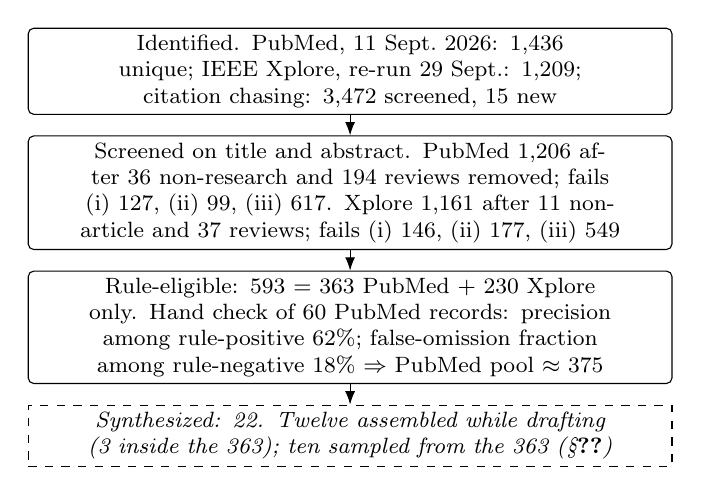
\begin{tikzpicture}[
  >=Latex, node distance=2.6mm,
  bx/.style={draw, rounded corners=2pt, align=center, text width=80mm, inner sep=2.5pt, font=\footnotesize},
  nr/.style={draw, dashed, align=center, text width=80mm, inner sep=2.5pt, font=\footnotesize\itshape}]
\node[bx] (a) {Identified. PubMed, 11 Sept.\ 2026: 1{,}436 unique; IEEE Xplore, re-run 29 Sept.: 1{,}209; citation chasing: 3{,}472 screened, 15 new};
\node[bx, below=of a] (d) {Screened on title and abstract. PubMed 1{,}206 after 36 non-research and 194 reviews removed; fails (i) 127, (ii) 99, (iii) 617. Xplore 1{,}161 after 11 non-article and 37 reviews; fails (i) 146, (ii) 177, (iii) 549};
\node[bx, below=of d] (e) {Rule-eligible: 593 $=$ 363 PubMed $+$ 230 Xplore only.
  Hand check of 60 PubMed records: precision among rule-positive 62\%; false-omission fraction among rule-negative 18\% $\Rightarrow$ PubMed pool $\approx$ 375};
\node[nr, below=of e] (f) {Synthesized: 22. Twelve assembled while drafting (3 inside the 363); ten sampled from the 363 (\S\ref{sec:selection})};
\foreach \u/\v in {a/d,d/e,e/f} {\draw[->] (\u) -- (\v);}
\end{tikzpicture}
\caption{Literature selection flow, with the counts logged when each query was run, in the PRISMA reporting convention~\cite{page2021prisma}. Exclusion reasons at the screening stage are the three criteria of Section~\ref{sec:method}: (i) no space--time or explicit longitudinal structure, (ii) no clinical or public-health task, (iii) no quantitative result against a named baseline. The endpoint differs from a systematic review: at the dashed box we sample for taxonomy coverage rather than carry the eligible set forward.}
\label{fig:prisma}
\end{figure}
Both IEEE Xplore arms were screened under the same rules: of the 1{,}209 records, 11 are non-article item types and 37 are reviews, leaving 1{,}161 screened on title and abstract; 177 failed~(ii), 146 failed~(i) and 549 failed~(iii), leaving 289, and 284 after deduplication within Xplore (5 records appear on both arms). Of these, 54 are already in the 29 September 2026 PubMed snapshot and 230 are Xplore only, so the rule-eligible literature across the two databases is 593 records rather than 363; the hand check covered the PubMed screen alone, so its correction is not carried across. The records were paged from the search endpoint 100 at a time and re-screened on 1 October 2026, when 271 of the 274 twin-arm rows exported on 22 September were returned again and the arms had grown to 277 and 932 records; because that endpoint truncates abstracts to about 400 characters, which made the truncated text yield \emph{zero} eligible records out of 913, the full abstract of every record was fetched before screening.

Xplore exposes no publication-type metadata, so reviews were removed by a textual rule---a title or the first 700 characters of the abstract presenting the work as a survey, review, overview, tutorial, scoping study or meta-analysis---which removed 37 records (18 and 19 by arm) and moved the eligible count only from 286 to 284; unlike the PubMed exclusion, it catches only a review that describes itself as one. Two records are the same when their digital object identifiers (DOIs) agree after lowercasing and stripping a trailing period, or when their titles agree after lowercasing and deleting every non-alphanumeric character; within Xplore the first occurrence is kept, and against PubMed a matched record is not added to the pool.

\subsection{Selection of the Synthesized Studies}
\label{sec:selection}
The 593 rule-positive records describe the output of the logged search and screen; the twenty-two studies of Table~\ref{tab:evidence} are a \emph{focused synthesis}, and no prevalence statement transfers from one to the other. The twenty-two have two provenances, which we keep distinct because they support different conclusions. Twelve were assembled while drafting earlier versions of this survey, before the searches were run; resolved by DOI only 3 of them are retrieved by the query, although the retained methodology states that all twelve are indexed in PubMed. The other ten were drawn from the 363 PubMed rule-eligible records under a stated frame: we crossed the five data types of Section~\ref{sec:data} with the clinical domains present in the pool, kept only records whose abstract names a body-worn, ambient or consumer device or an edge deployment, and within each empty cell took the record that added a device class or a task not already represented, stopping when three consecutive candidates added no new data type, model family, domain or IoT layer. That saturation rule, not a target count, fixed the number at ten, and Table~\ref{tab:evidence} is therefore an illustrative set assembled by the authors, not a representative sample of the literature the search sizes. The IEEE Xplore arm was screened only after the set was fixed and contributed no study to Table~\ref{tab:evidence}'s twenty-two, so the 230 Xplore-only records---which are where IoT-native engineering work concentrates---were assessed in a separate second-stage screen (Section~\ref{sec:iotcomplement}) whose retained records are reported beside, not inside, the twenty-two. The extraction records describe full-text assessment for 21 studies; the summary for Nitski et al. is restricted to its accessible abstract and does not support a detailed assessment of its complete evaluation protocol. One further candidate, J.~Xie and B.~Yao, \emph{Comput.\ Biol.\ Med.}, vol.~146, p.~105586, 2022, could not be obtained and was dropped rather than described from its abstract.

For the full-text-assessed studies, the extraction covered dataset descriptors, ten quality fields (split, leakage risk, missing data, external validation, calibration and uncertainty, subgroups, comparators, reproducibility, clinical validation), deployment and privacy reporting, and results with the available comparator on the stated metric and protocol. The abstract-only record was limited to information available in that abstract. Every table of this survey is in the article itself (Tables~\ref{tab:related-surveys}--\ref{tab:agenda-a}); nothing is deferred to a supplement. The records behind them are released as a separate audit package of data files, named A01--A14 so that no file can be confused with a numbered table, and listed in a manifest with dates and checksums: survey-comparison coding (A01), study provenance and reasons for inclusion (A02), dataset, quality and deployment fields (A03--A07), a crosswalk from the stable identifiers E01--E22 and C1--C7 to every table row (A08), the record-level PubMed and Xplore screening decisions with duplicate matches (A09--A10), the hand check (A11), the IoT-complement screen (A12), the 22 October search update (A13), and the screening code and dated query logs (A14). The package is deposited at \url{https://github.com/Xin-Ray/survey} under \texttt{expand25/audit/}, its manifest giving each file's date and SHA-256 prefix so a reader can verify the copy obtained.

\subsection{Citation Chasing and Search-Term Sensitivity}
\label{sec:chasing}
Forward and backward citation chasing was run through OpenAlex from ten of the twelve reviews then in Table~\ref{tab:related-surveys} whose records carry a reference list or citing works (the other two have none; the three 2026 additions postdate the chase), screening 3{,}472 distinct records under the same criteria and surfacing 15 eligible ones that the PubMed query had missed: backward, 1{,}523 references gave 1{,}362 retrievable records and 1 eligible; forward, 3{,}120 citing works fetched under a cap of 400 per seed gave 2{,}110 distinct records and 14 eligible. Most were rejected for lacking a spatial or temporal term (1{,}184 backward, 1{,}909 forward). The count is a lower bound: three seeds reached the cap, OpenAlex lacks many abstracts, and most of the fifteen are activity-recognition papers citing the wearable-sensing review.

Block C names only two IoT terms, \emph{wearable} and \emph{wearables}. To size what this misses, we re-ran the PubMed spatiotemporal arm on 16 October 2026 with an IoT block---Internet of Things, IoT, sensor(s), smartphone(s), mHealth, mobile health, edge computing, body area network and remote monitoring---added by OR to block C: the arm grew from 1{,}194 to 1{,}501 records, so 307 records (26\%) carry an IoT term but no health term; repeated on 22 October 2026 (Fig.~\ref{fig:strings}) it gave 1{,}198 and 1{,}505, again 307 added records, which were screened as described next.

\subsection{IoT-Engineering Complement Screen}
\label{sec:iotcomplement}
The 230 Xplore-only rule-positive records and the 307 IoT-term additions were screened on 22 October 2026 in two stages, with one decision per record (audit file A12). The IoT-term records first met the item-type exclusion and criteria (i)--(iii); 68 of 307 passed. A second textual stage kept records that (E1) take data from a body-worn, ambient, smartphone, camera or other connected device and (E2) report or evaluate a system quantity---latency, energy, memory, model size, bandwidth, or on-device or edge execution---leaving 37 Xplore-only and 21 IoT-term candidates. Each candidate's abstract was then assessed, with AI assistance and a recorded reason per record for author verification, and a record was retained only when it addressed a human health endpoint and gave a quantitative system figure; 52 were excluded with a stated reason, most often a non-health task (security, environment, manufacturing, or activity and gesture recognition without a clinical endpoint) or a system claim without a figure. Six were retained, and the search update below added a seventh (C1--C7, Table~\ref{tab:evidence}). They are extracted from abstracts, are not added to the twenty-two, and enter Fig.~\ref{fig:heatmap} only through its separately marked c cells. They sharpen the resource column without supplying what the twenty-two lack: recurrent, distilled and state-space models report latency or size reductions, but only one names and measures its hardware---an event-driven convolutional classifier on a 40\,nm compute-in-memory chip, 5\,$\mu$s and 100--150\,$\mu$J per beat~\cite{raghuraman2026cimecg}---and none states a subject-level split or reports calibration.

\subsection{Search Update Through 22 October 2026}
\label{sec:searchupdate}
Both databases were re-searched on 22 October 2026 with the strings of Fig.~\ref{fig:strings}, and online dates were logged per record (audit file A13). PubMed records first indexed between 12 September and 22 October (Entrez date) numbered 50; 18 were reviews or non-research items and 9 passed criteria (i)--(iii). The Xplore arms returned 961 and 289 records; the 44 inserted after the 22 September export gave 12 rule-positive records, and the Xplore-only rule-positive set grew from 230 to 242. Under the selection frame of Section~\ref{sec:selection}, the 21 new rule-positive records were assessed like the complement candidates: one met E1, E2 and the health-endpoint test and was added as C7, and the rest were excluded with reasons (twin-labelled retrospective pipelines without a measured figure, single-subject feasibility platforms, or non-device tasks). The re-run also settled the question of the 54 cross-database overlaps, which had been matched against the full PubMed snapshot rather than the rule-eligible pool: re-identified, 54 of the 55 matched records are in the 363-record pool, and one fails criterion (iii) on its PubMed abstract, so the combined rule-positive count is 593 with PubMed's verdict and 594 if either database's verdict sufficed. The twenty-two are unchanged.

\subsection{Reporting Principles: What the Search and the Synthesis Can Establish}
\label{sec:scopeaudit}
Five principles govern how the evidence is reported, and later sections rely on them rather than repeating them.

\emph{One document, no supplement.} Every table and figure the argument uses is in this article; there is no supplementary document, and no claim depends on material outside it. Records too detailed for a table---per-study fields, record-level screening decisions, code and dated query logs---are released only as the data files A01--A14 of Section~\ref{sec:selection}, which carry the same study identifiers as the tables and add no result that the article does not state.

\emph{Separate denominators.} The 593 records passed title-and-abstract rules in the retained snapshots; they are not 593 studies confirmed eligible by full-text assessment, and the hand check of sixty PubMed records measures one author's disagreement with a textual rule (21 rule-positive and 39 rule-negative records), not inter-rater agreement or the true eligible count, and it is not independent of the automated pipeline it checks. The twenty-two are an illustrative set: thirteen are linked to the rule-eligible pool by the recorded procedure (the ten sampled and three of the twelve drafting-stage selections), and the other nine must not be read as a sample of the search output. Complement records (C1--C7) and the twin and world-model examples of Sections~\ref{sec:DT}--\ref{sec:world_model_dt} are never added to this denominator.

\emph{Conditional statements.} A coded property is reported as found, or not established, in the illustrative set under the stated extraction; no prevalence in the wider field is estimated. The absence of an untouched external test here is a reason to ask more of these studies, not evidence that the engineering literature contains none. Two records are contextual rather than tests of a deep network against a baseline: the county-prevalence analysis is a statistical reference for regional structure and uncertainty, and the embedded stride study supplies instrument agreement and a memory footprint but no same-data comparator.

\emph{Non-reporting is not negative evidence.} A field is coded as demonstrated only when the cited evaluation supports it directly; an unfavorable result means worse on a stated outcome and protocol; an unreported result means no supporting measurement in the assessed material; and an unclear protocol stays unclear. Another cohort's name does not establish an untouched transfer test, and an abstract identifies an endpoint without establishing leakage, calibration or external validity. Intervals on performance or predictions are never treated as calibration.

\emph{Replay, not reconstruction.} The saturation rule states the authors' selection rationale but, without a candidate-by-candidate ordering, cannot be replayed to its stopping point, so it is not a claim that every model family or IoT deployment was captured. Database counts drift as records are indexed; a re-run of the same strings (Section~\ref{sec:searchupdate}) is a sensitivity check and an update, not a reconstruction of the historical snapshot. A record-level replay of the PubMed screen restricted to records indexed by 11 September (audit file A09) returns 1{,}435 of the 1{,}436 records and 363 rule-positive records, 356 of them in the original pool; the original run kept only aggregate counts, so the residual differences cannot be traced further. Method papers can establish computational structure but cannot supply patient-level validation for a family.

\section{Spatiotemporal Data in Connected Digital Health}
\label{sec:data}
\begin{figure*}[tp]
\centering
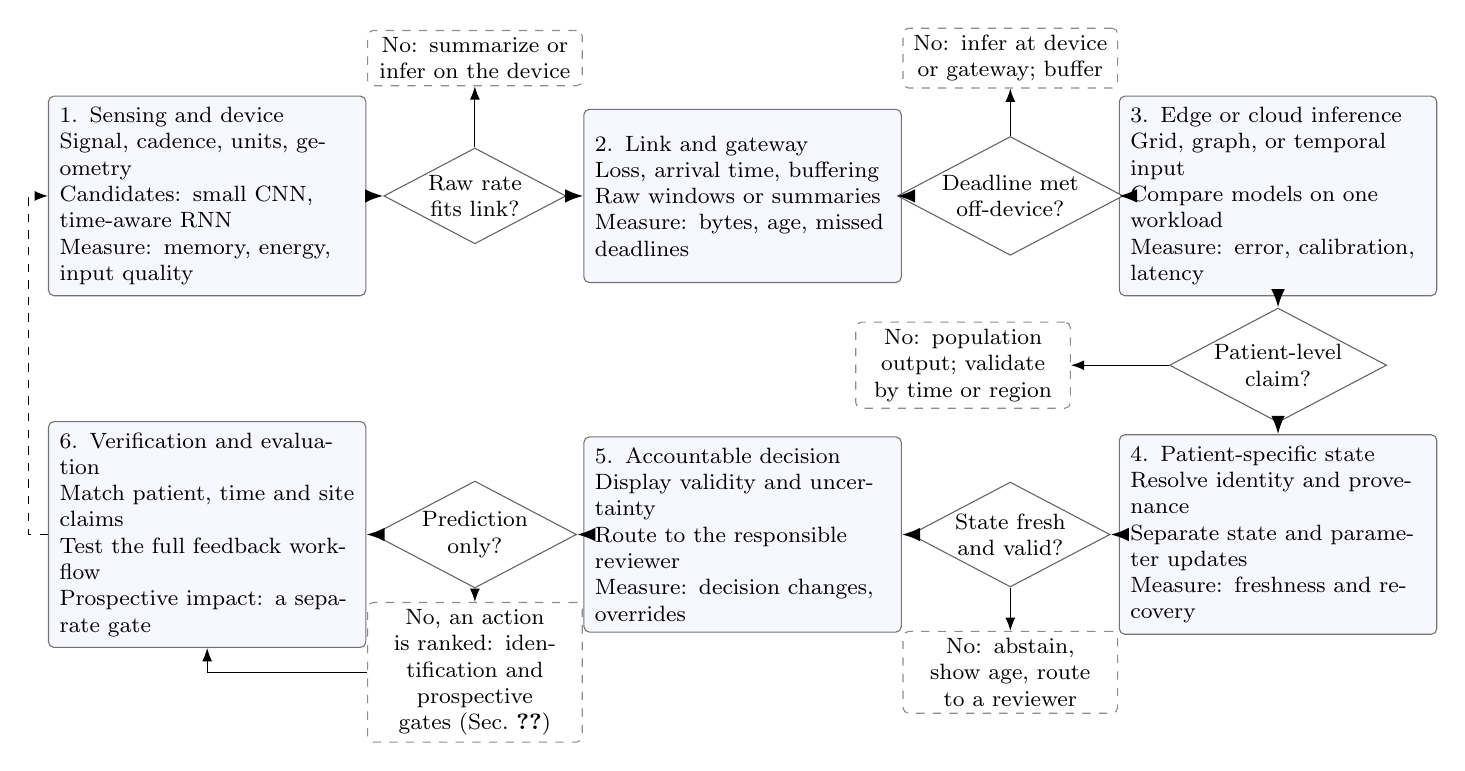
\begin{tikzpicture}[>=Latex,font=\footnotesize,
box/.style={draw=black!55,rounded corners=2pt,fill=blue!3,text width=3.75cm,minimum height=2.2cm,align=left,inner sep=4pt},
dec/.style={draw=black!60,diamond,aspect=1.9,inner sep=0.6pt,align=center,fill=white,font=\footnotesize},
alt/.style={draw=black!45,dashed,rounded corners=2pt,align=center,inner sep=2.5pt,text width=2.55cm,font=\footnotesize}]
\node[box] (s) at (0,0) {1. Sensing and device\\Signal, cadence, units, geometry\\Candidates: small CNN, time-aware RNN\\Measure: memory, energy, input quality};
\node[box] (g) at (6.8,0) {2. Link and gateway\\Loss, arrival time, buffering\\Raw windows or summaries\\Measure: bytes, age, missed deadlines};
\node[box] (e) at (13.6,0) {3. Edge or cloud inference\\Grid, graph, or temporal input\\Compare models on one workload\\Measure: error, calibration, latency};
\node[box] (t) at (13.6,-4.3) {4. Patient-specific state\\Resolve identity and provenance\\Separate state and parameter updates\\Measure: freshness and recovery};
\node[box] (c) at (6.8,-4.3) {5. Accountable decision\\Display validity and uncertainty\\Route to the responsible reviewer\\Measure: decision changes, overrides};
\node[box] (v) at (0,-4.3) {6. Verification and evaluation\\Match patient, time and site claims\\Test the full feedback workflow\\Prospective impact: a separate gate};
% decision branches
\node[dec] (d1) at (3.4,0) {Raw rate\\fits link?};
\node[dec] (d2) at (10.2,0) {Deadline met\\off-device?};
\node[dec] (d3) at (13.6,-2.15) {Patient-level\\claim?};
\node[dec] (d4) at (10.2,-4.3) {State fresh\\and valid?};
\node[dec] (d5) at (3.4,-4.3) {Prediction\\only?};
\node[alt] (a1) at (3.4,1.75) {No: summarize or infer on the device};
\node[alt] (a2) at (10.2,1.75) {No: infer at device or gateway; buffer};
\node[alt] (a3) at (9.6,-2.15) {No: population output; validate by time or region};
\node[alt] (a4) at (10.2,-6.05) {No: abstain, show age, route to a reviewer};
\node[alt] (a5) at (3.4,-6.05) {No, an action is ranked: identification and prospective gates (Sec.~\ref{sec:world_model_dt})};
\draw[->,thick] (s)--(d1); \draw[->,thick] (d1)--(g);
\draw[->,thick] (g)--(d2); \draw[->,thick] (d2)--(e);
\draw[->,thick] (e)--(d3); \draw[->,thick] (d3)--(t);
\draw[->,thick] (t)--(d4); \draw[->,thick] (d4)--(c);
\draw[->,thick] (c)--(d5); \draw[->,thick] (d5)--(v);
\draw[->] (d1)--(a1); \draw[->] (d2)--(a2); \draw[->] (d3)--(a3); \draw[->] (d4)--(a4); \draw[->] (d5)--(a5);
\draw[->] (a5.west) -| (v.south);
\draw[->,dashed] (v.west) -- ++(-.25,0) |- (s.west);
\end{tikzpicture}
\caption{Proposed sensing-to-decision framework. Each stage links an acquisition or deployment choice to the measurements needed to evaluate it. Diamonds are the design decisions that route a deployment between stages; the main path is taken on yes, and the dashed box gives the branch taken on no. Arrows describe the workflow; they do not assert that the complete loop was demonstrated by the 22 illustrative studies.}
\label{fig:taxonomy}
\end{figure*}

\subsection{Five Data Types and Where They Enter the Pipeline}
\begin{figure}[tp]
\centering
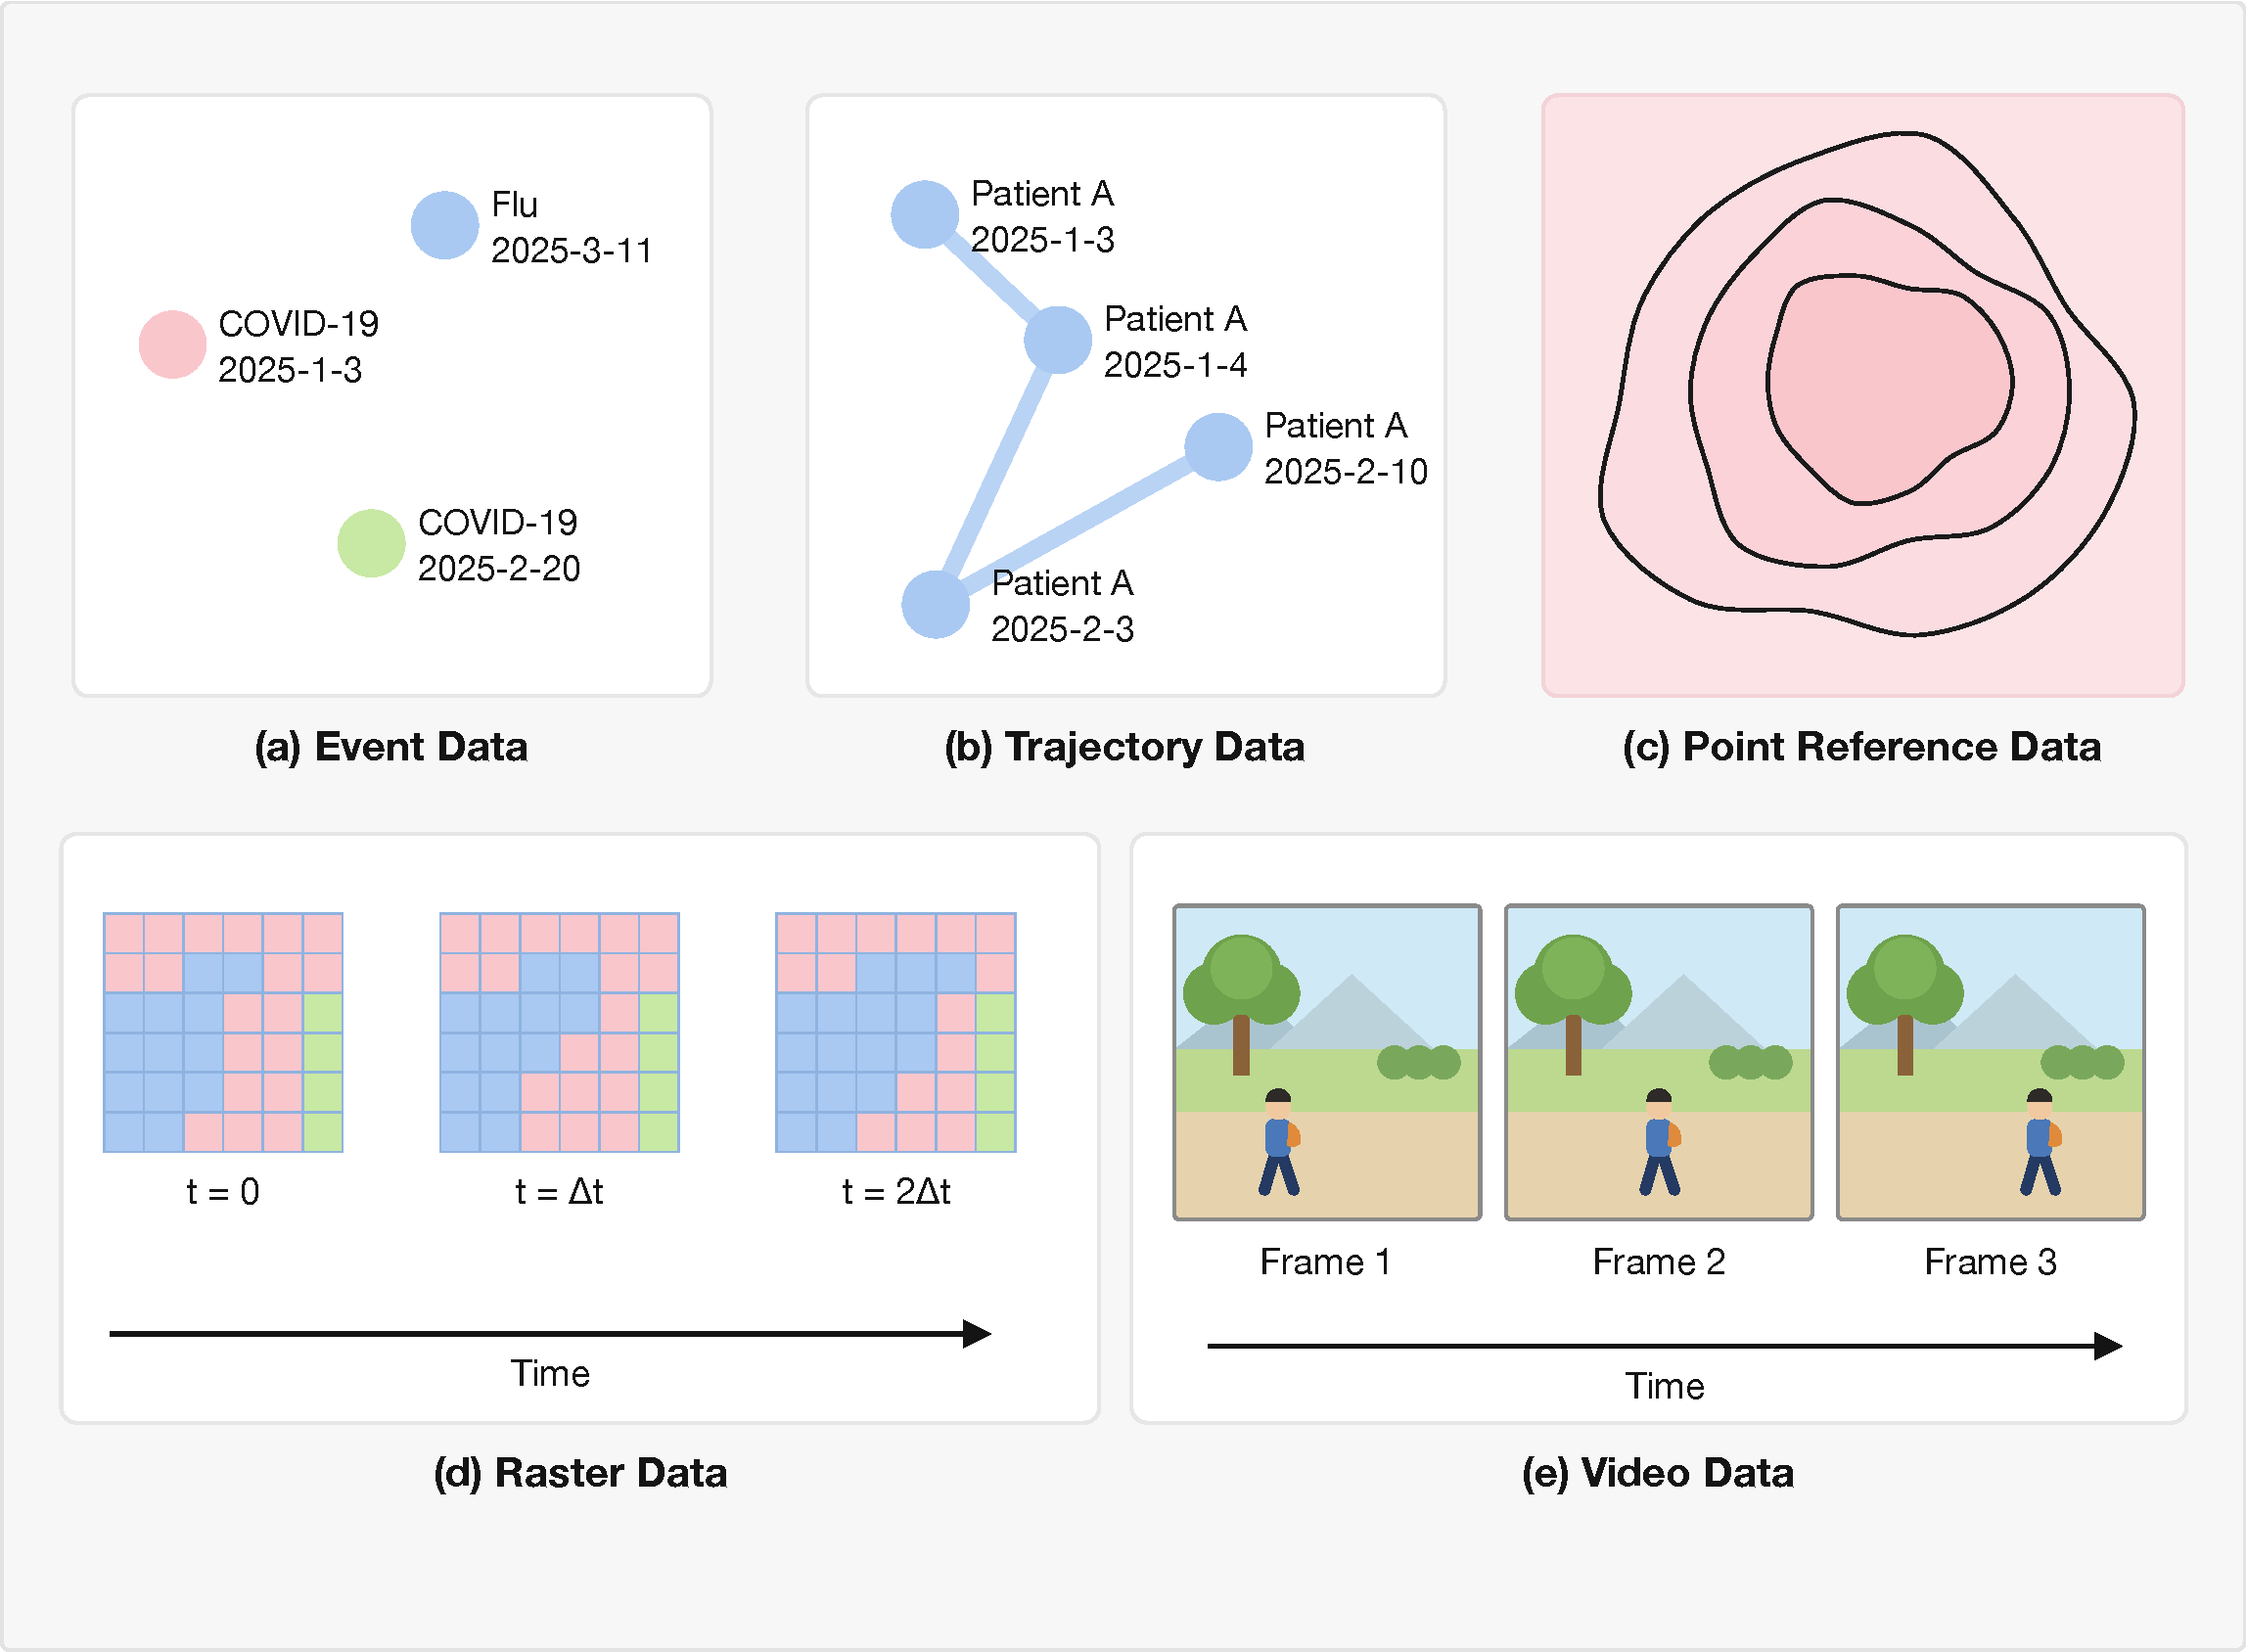
\includegraphics[width=\linewidth]{fig3.pdf}
\caption{The five spatiotemporal data types of connected digital health, each with the record form it takes: (a) sparse events; (b) an ordered trajectory; (c) series at fixed sites; (d) a raster, the same gridded spatial field observed at regular times; (e) video, an ordered sequence of image frames. Relational structure---brain connectivity, referral or sensor networks---is a layer over these types, not a sixth type.}
\label{fig:fivecat}
\end{figure}
Following prior work~\cite{wang2022deep,atluri2018stdm}, spatiotemporal health data fall into five types, each entering the connected pipeline of Fig.~\ref{fig:taxonomy} at a different point (Fig.~\ref{fig:fivecat}). \emph{Event} data are discrete (location, time, type) records such as outbreak reports or on-device alarms, arriving sparsely over low-bandwidth links. \emph{Trajectory} data are ordered (location, time) series from wearables or mobile units, sampled continuously and summarized before transmission. \emph{Point reference} data are measurements at known locations, such as air quality or heart rate, from ambient, home and clinic instruments. \emph{Raster} data occupy fixed locations at regular intervals, forming a space--time tensor from server-side aggregation or volumetric imaging, functional magnetic resonance imaging (fMRI) included. \emph{Video} data are frame sequences from ultrasound, endoscopy and ward cameras, whose bandwidth forces edge processing or selective upload. Data type, achievable sampling rate and feasible inference location are thus fixed together by the deployed sensing tier, and what that tier can execute is a hardware question as much as a modeling one: microcontroller-class learning is practical at wearable scale~\cite{saha2022mcuml}, and one study here runs an int8 network in 14\,kB of random-access memory (RAM)~\cite{verbiest2023gaitstride}. Relational structure---brain connectivity, referral or sensor networks---is a layer over these types rather than a sixth, and it is what spatiotemporal graph neural networks (STGNNs) consume.

\subsection{What Counts as Spatial Modeling}
\label{sec:spatial}
``Spatiotemporal'' covers inputs that differ in kind, and the evidence cannot be read without separating them. We code each study by the spatial structure its \emph{model} uses: geographic coordinates (Geo); administrative regions (Adm); an anatomical, voxel or image grid (Anat); an explicit relational layout of sensors or body segments that the model encodes (Rel); several channels with no spatial relation encoded (MC); or no spatial structure, so the evidence is temporal or longitudinal only (T). Of the twenty-two studies, two use administrative regions, five an anatomical or image grid and three a relational layout---ten in all that model space explicitly---while five are multichannel without a spatial prior and seven are temporal only (Table~\ref{tab:evidence}). None uses geographic coordinates, and no dataset carries the position of a person or device in a built environment, even though place-based exposure motivates much of the field. Multichannel and temporal-only studies are kept in the synthesis because the connected pipeline produces them, but they are not evidence that modeling space helps.

\subsection{IoT Status, Irregularity and Missingness}
\label{sec:iotstatus}
We also code, as each study's evidence class, whether the data are \emph{IoT-native}---captured by a body-worn, ambient or consumer device that a deployment would use (N, eleven studies); \emph{IoT-adaptable}---acquired with a clinical instrument whose signal has a portable form, such as electroencephalography (EEG) or magnetocardiography (A, three); or \emph{record-based}---scanner imaging, registry or survey data that do not themselves establish a live IoT acquisition stream (R, eight). These are acquisition codes, not evidence of an operating networked service. Device readiness is not inferred from architectural complexity: a model counts as running on a device only where the study measured it there.

Acquisition explains much of the irregularity the models must handle. Health data are sparse and irregularly sampled, with missingness from non-compliance or operational limits~\cite{che2018grud} and site-specific schedules producing uneven intervals that violate standard temporal assumptions unless gaps are modeled explicitly~\cite{shukla2021irregular}. In IoT-native data the gaps have device causes---a flat battery, a removed wearable, a lost link, a broker that drops a message---which make missingness informative of the patient's own behavior; in record-based data the gaps follow the visit protocol. Where the studies state how missingness was handled they impute---by interpolation, forward or backward filling, or the training mean---or exclude records or subjects; eight state nothing, and none models missingness as a function of the device or the link.

\subsection{Data Quality and Harmonization}
Before joint modeling the data must be made comparable, and the reviewed studies report this unevenly: sensor calibration and drift at the device level; clock skew and preprocessing that can leak information if future observations or test-fitted parameters are used; aggregation units and boundary changes at the spatial level; and site shift, identity resolution across a participant's devices and schema interoperability at the system level, where the Health Level Seven (HL7) Fast Healthcare Interoperability Resources (FHIR)~\cite{ayaz2021fhir} and the IEEE 11073 device profiles~\cite{ieee11073std} are the usual anchors. Harmonized multi-site efforts show what is possible: iPAT aligns measurements with time indexes and site-level metadata across national trials~\cite{Fang2021iPAT}, and UK Biobank standardized acquisition and follow-up across its assessment centers~\cite{sudlow2015ukbiobank}.

\subsection{Datasets Underlying the Synthesized Studies}
\label{sec:datasets}

Table~\ref{tab:datasets} describes the twenty-three dataset-description rows for the twenty-two studies; some rows combine cohorts and one study occupies two rows. Fourteen carry a continuous stream at a sensor rate, from 1\,Hz heart rate to intracranial EEG sampled at up to 5\,kHz, but only nine of those come from a body-worn, ambient or consumer device; the remaining nine are visit-, scan- or month-indexed. The largest populations are registries sampled on a clinic schedule, so population size and temporal resolution trade off across the set, and these descriptors do not establish a dataset that validates the complete sensor-to-decision workflow.

\begin{table*}[tp]
\centering
\caption{Dataset-description rows underlying the twenty-two illustrative studies. Some rows combine cohorts; the 23 rows are not 23 independent datasets. Entries and access conditions are as reported, not newly verified availability; ``n/r'': not reported. Sp.: spatial structure the study's model uses (Section~\ref{sec:spatial}).}
\label{tab:datasets}
\footnotesize
\setlength{\tabcolsep}{2.5pt}
\renewcommand{\arraystretch}{1.12}
\begin{tabularx}{\textwidth}{|>{\raggedright\arraybackslash}p{3.6cm}|>{\raggedright\arraybackslash}p{3.0cm}|X|>{\raggedright\arraybackslash}p{2.6cm}|>{\raggedright\arraybackslash}p{0.75cm}|>{\raggedright\arraybackslash}p{0.65cm}|>{\raggedright\arraybackslash}p{1.6cm}|>{\raggedright\arraybackslash}p{0.95cm}|}
\hline
Dataset (ID, study) & Population & Signal; device & Sampling; duration & Sp. & Fit & Access & Ref. \\
\hline
FIC intake cycles (E03 Kyritsis et al.) & 12 subjects, 21 meals & Wrist inertial; smartwatch & 100\,Hz; one meal & T & D & Public & \cite{Kyritsis2019EatingBehavior} \\
\hline
MODMA EEG (E12 Liu et al.) & 53 subjects, 24 depressed & EEG; 128-channel net & 250\,Hz & Anat & -- & On application & \cite{2} \\
\hline
OpenNeuro ds002748 (E13 Zhang et al.) & 72 subjects, 51 depressed & Resting-state fMRI; 3\,T & TR 2.5\,s; 6\,min & Anat & -- & Public & \cite{9} \\
\hline
Two-site fMRI (E14 Kong et al.) & 277 subjects, two hospitals & Resting-state fMRI and T1; 3\,T & TR 2\,s; 8\,min & Rel & M & Private & \cite{4} \\
\hline
Thai district counts (E18 Thaipisutikul et al.) & 13 districts and national & Depression case counts; surveillance & Monthly; 70 points & Adm & -- & Public & \cite{3} \\
\hline
UVA/Padova, ABC4D, OhioT1DM (E01 Li et al.) & 20 virtual; 10 and 6 with type 1 diabetes & CGM, insulin, meals; Dexcom CGM & 5\,min; 8\,wk--180\,d & T & D, T & Mixed & \cite{Li2020GluNet} \\
\hline
Life-log CGM cohort (E02 Lim et al.) & 171 healthy adults & CGM and app log; Dexcom G7 & 15\,min; $\geq$12\,d & T & D, T & Not public & \cite{Lim2025VirtualCGM} \\
\hline
BRFSS and ACS counties (E19 Li et al.) & 3109 counties, 48 states & Survey prevalence and covariates & Annual, 2004--2011 & Adm & -- & Public & \cite{XiaoLi2016DiabetesSpatiotemporal} \\
\hline
Multicentre aortic CMR (E17 Bohoran et al.) & 376 patients, 424 scans & Cine CMR; 4 scanners, 3 centers & One cardiac cycle & Anat & M & On request & \cite{5} \\
\hline
ADNI (E20 Lin and Luo) & 1068 with mild cognitive impairment & Clinical and imaging-derived visits & 6--12\,mo; mean 3.3\,y & T & M & On application & \cite{lin2022deep} \\
\hline
NACC (E20 Lin and Luo) & 5261 with mild cognitive impairment & Clinical visit variables & About annual; 2.8\,y & T & M & On application & \cite{lin2022deep} \\
\hline
SRTR and UHN (E21 Nitski et al.) & 42\,146 and 3269 transplant recipients & Registry and laboratory records$^{\S}$ & 1--12\,mo; 5.8--8.0\,y$^{\S}$ & T & M & On request; no$^{\S}$ & \cite{nitski2021long} \\
\hline
Health ABC DXA (E22 Glaser et al.) & Over 3000 adults, 15\,000 scans & Whole-body DXA, exam data & Up to 8 visits, 16\,y & Anat & -- & On request & \cite{glaser2022deep} \\
\hline
Cuffless-BP cohorts (E04 Liu et al.) & 305 subjects, three cohorts & ECG and PPG; clinical monitors & 1\,kHz; 10\,min & MC & D & Partly public & \cite{liu2024cignn} \\
\hline
SERF magnetocardiography (E16 Li et al.) & 2118 subjects, 983 with ischemia & Single-channel MCG; optically pumped magnetometer & One cardiac cycle & T & -- & Private & \cite{li2026edgeischemia} \\
\hline
Foot IMU strides (E05 Verbiest et al.) & 15 healthy adults, 4467 strides & Foot IMU with Cortex-M4F; OptoGait reference & 102.4\,Hz & T & D & n/r & \cite{verbiest2023gaitstride} \\
\hline
WearGait-PD (E06 Herath et al.) & 181 subjects, 100 with Parkinson's & Body-worn IMUs; Movella DOT & 100\,Hz; walking bouts & Rel & D & Public & \cite{herath2026parkinson} \\
\hline
Smart-bed array (E07 Liu et al.) & 30 healthy adults & Accelerometer array in a mattress & 240\,Hz; staged postures & Rel & D & On request & \cite{liu2025sleepposture} \\
\hline
Sit-to-stand videos (E08 Chan et al.) & 309 participants, 2063 videos & Smartphone video, pose & 30\,Hz & MC & D & n/r & \cite{chan2026sitstand} \\
\hline
Exercise cohort (E09 Wang et al.) & 21 adults & Heart rate, acceleration, gas exchange & 1\,Hz; graded test & MC & D & On request & \cite{wang2025vo2} \\
\hline
VIPL-HR (E10 Zhu et al.) & Public face-video set & Color face video; webcams & 25 frames/s & Anat & D & Public & \cite{zhu2024ippg} \\
\hline
Ninapro DB2 (E11 Lin et al.) & 40 subjects, 40 movements & Surface EMG array, data glove & 2\,kHz & MC & D & Public & \cite{lin2024smapen} \\
\hline
CHB-MIT; Kaggle AES and Melbourne (E15 Hussein et al.) & 22 scalp-EEG patients; intracranial: 5 dogs, 5 patients & Scalp and intracranial EEG; clinical systems & 256\,Hz to 5\,kHz & MC & M & Public & \cite{hussein2022seizure} \\
\hline
\multicolumn{8}{@{}>{\raggedright\arraybackslash}p{\dimexpr\textwidth-4\tabcolsep\relax}@{}}{\footnotesize Fit denotes potential research use, not a demonstrated service: D device/edge evaluation; M multisite evaluation; T longitudinal patient-state research; -- not assigned. These labels do not establish synchronization or intervention effects. E01--E22: stable study identifiers shared with Table~\ref{tab:evidence} and the audit files. $^{\S}$Nitski et al.\ is assessed from its abstract, which confirms the two cohorts and their sizes; the marked descriptors come from the earlier extraction and are not verified here. Sp.: Adm administrative regions; Anat anatomical, voxel or image grid; Rel relational sensor layout encoded by the model; MC multichannel without a spatial prior; T temporal only. EEG: electroencephalography. fMRI: functional magnetic resonance imaging; TR: repetition time. CGM: continuous glucose monitoring. BRFSS: Behavioral Risk Factor Surveillance System; ACS: American Community Survey. CMR: cardiovascular magnetic resonance. ADNI: Alzheimer's Disease Neuroimaging Initiative; NACC: National Alzheimer's Coordinating Center. SRTR: Scientific Registry of Transplant Recipients; UHN: University Health Network. DXA: dual-energy X-ray absorptiometry. BP: blood pressure; ECG: electrocardiography; PPG: photoplethysmography. SERF: spin-exchange relaxation-free; MCG: magnetocardiography. IMU: inertial measurement unit. EMG: electromyography. AES: American Epilepsy Society.}
\end{tabularx}
\end{table*}

\subsection{The Acquisition Contract and Availability}
\label{sec:acquisitioncontract}
\label{sec:availability}
An acquisition contract states what can reach the model: channels, units, precision, sampling and arrival times, sensor geometry, window length and expected gaps. A regular array supports a convolutional prior and a known relation a graph; channel multiplicity alone supports neither, which is why EEG brain maps, functional-connectivity graphs and joint-angle sequences receive different spatial codes. Geometry used in preprocessing differs from geometry encoded by the predictor---a pose extractor can use anatomy while the downstream model treats its outputs as independent channels---and a replacement sensor or montage can change both signal meaning and topology, so evaluation should test the deployed contract rather than matching array dimensions. The contract also fixes the information set: a glucose forecast from previous CGM, glucose inference without current CGM and a risk update at a visit answer different questions, and their errors cannot rank architectures.

Missingness enters at several stages---no sample acquired, a late packet, a failed preprocessing step, a rejected input---and the remedies differ: retransmission recovers a stored packet but not an unmeasured observation, and imputation does not show that the mechanism is harmless. A replay should keep acquisition and arrival timestamps, masks and outages, fit imputation and normalization on training data only, and report error against gap duration and observation age together with the fraction of intended opportunities that yield a valid output. Availability can differ by device ownership, mobility, lighting and gateway access, so complete-case evaluation can change the target population; the artificial independent noise tested by sMAPEN is narrower than block outages, device shift or nonrandom adherence. These are evaluation requirements, not measurements recovered for every illustrative study.

\section{Deep Learning--Based Spatiotemporal Modeling Methods for Connected Health}
\label{sec:history}
This section introduces notation alongside the models, then separates what each family assumes and costs in principle from what the reviewed studies have measured. Several architectures were first demonstrated on traffic or climate sensing, a task of the same shape---distributed sensors at irregular rates over a non-Euclidean topology, bursty missingness, inference under bandwidth and energy limits---but health adds subject-level identifiability, informative missingness and small cohorts, so a transferred architecture must be re-validated on patients.

\subsection{Historical Development}

Spatiotemporal deep learning in healthcare moved from feed-forward models with hand-engineered spatial context~\cite{miotto2018deeplearning} to graph convolution for non-Euclidean relations and attention for long-range dependence~\cite{caroprese2018deepehr}, and since 2020 to Transformers, self-supervised learning and multimodal fusion~\cite{sun2026irregularmedical}. The statistics literature supplied interpretable covariance structure and principled baselines for irregular, nonstationary locations, including physics-informed convection--diffusion models and statistical deep learning syntheses~\cite{liu2022convectionDiffusion,wikle2023statisticalDeepLearning}; these remain the baselines against which a neural model's added complexity should be justified.

\subsection{Foundational Architectures}
\label{sec:foundations}
\begin{figure*}[tp]
\centering
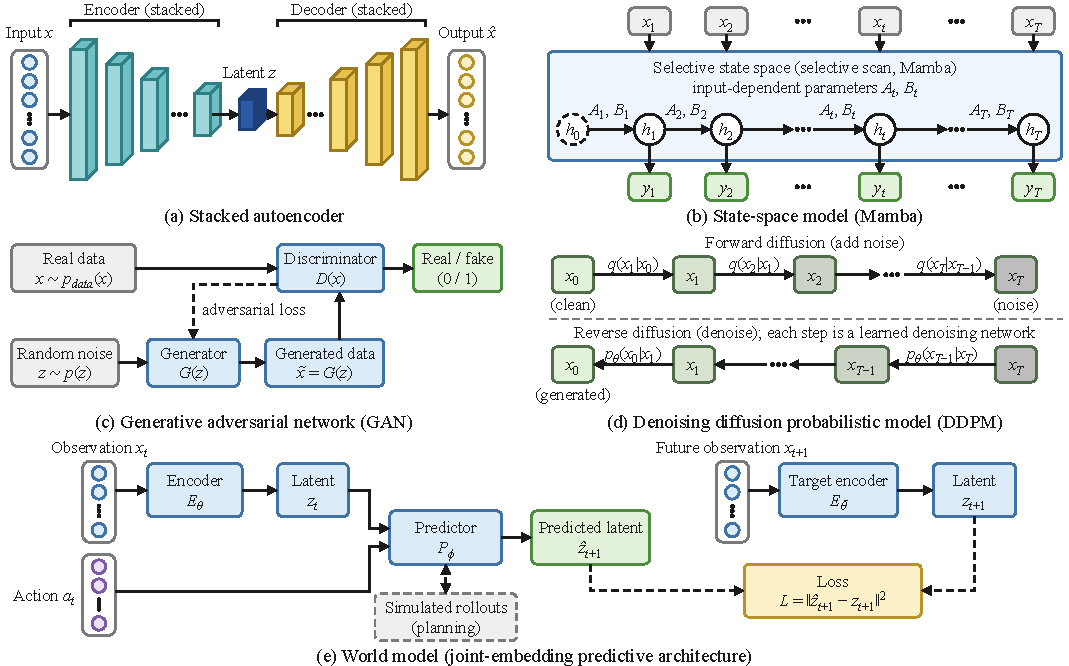
\includegraphics[width=\textwidth]{fig4_arch.pdf}
\caption{Internal structure of five foundational architectures. (a) The stacked autoencoder compresses an input into a latent code and reconstructs it; (b) the state-space model (Mamba) propagates an input-dependent hidden state through a selective scan; (c) the generative adversarial network (GAN) trains a generator against a discriminator; (d) the denoising diffusion probabilistic model (DDPM) learns to reverse a forward noising process; and (e) the world model encodes an observation into a latent state, predicts the next latent state from it and an action, and aligns the prediction with a target encoding of the future observation, as in~\eqref{eq:wm}.}
\label{fig:foundation_arch}
\end{figure*}
Figure~\ref{fig:foundation_arch} shows the generative and latent-dynamics architectures. Graph neural networks~\cite{scarselli2009gnn} process a graph $G=(V,E)$ by message passing,
\begin{equation}
m_i^{(l)} = \sum_{j \in \mathcal{N}(i)} f\bigl(h_j^{(l-1)}, h_i^{(l-1)}, e_{ij}\bigr), \quad h_i^{(l)} = \sigma\bigl(W m_i^{(l)} + b\bigr),
\label{eq:gnn}
\end{equation}
with the graph convolutional network (GCN)~\cite{kipf2017gcn} and the graph attention network (GAT)~\cite{velickovic2018gat} differing in aggregation. Recurrent networks~\cite{rumelhart1986rnn} carry a hidden state through time, with long short-term memory (LSTM)~\cite{rnn_lstm} and gated recurrent unit (GRU)~\cite{cho2014gru} gates against vanishing gradients; the Transformer~\cite{vaswani2017attention} replaces recurrence with self-attention at quadratic cost in sequence length. Autoencoders~\cite{hinton2006reducing} learn latent codes for anomaly detection and imputation; state-space models such as Mamba~\cite{gu2023mamba} propagate an input-dependent latent state in linear time, which motivates evaluating them on long CGM, electrocardiography (ECG), or EEG streams; linear sequence complexity alone does not establish suitability for a device; and generative adversarial networks~\cite{goodfellow2014gan} and diffusion models~\cite{ho2020ddpm} synthesize signals and impute. World models learn how an environment evolves so that actions can be evaluated by simulation~\cite{ha2018worldmodels}; joint-embedding predictive architectures~\cite{lecun2022jepa,maes2026leworldmodel} encode $x_t$ to $z_t$ and predict the next latent state under action $a_t$,
\begin{equation}
\begin{aligned}
z_t &= E_\theta(x_t), \quad \hat{z}_{t+1} = P_\phi(z_t, a_t),\\
L &= \bigl\| \hat{z}_{t+1} - E_{\bar{\theta}}(x_{t+1}) \bigr\|^2 .
\end{aligned}
\label{eq:wm}
\end{equation}
Here an action-conditioned latent transition is the formulation considered for planning. State-space models can also include control inputs, so the action argument does not define a mutually exclusive model class and does not make the predicted effects causal (Section~\ref{sec:causal}).

\subsection{Spatiotemporal Model Families}
\label{sec:families}
Four families recur in spatiotemporal health modeling. \emph{Convolutional--recurrent (CNN--RNN) hybrids} encode each gridded snapshot $X_t$ with a convolutional neural network (CNN) and the feature sequence with a recurrent neural network (RNN), or move the convolution inside the LSTM gates as ConvLSTM does~\cite{shi2015convolutional}; they assume a regular grid and learn long-range dependence poorly. \emph{Spatiotemporal graph neural networks}~\cite{shao2022longterm} treat sensors, hospitals or brain regions as nodes and alternate the aggregation of~\eqref{eq:gnn}, with edge weights or attention coefficients $\alpha_{ij}$, with recurrent, temporal-convolution or attention layers, as in DCRNN~\cite{li2018dcrnn}, STGCN~\cite{yu2018spatio} and Graph WaveNet~\cite{wu2019graphwavenet}; most assume a static topology, which a body area network whose devices join and leave violates. \emph{Transformer-based models} attend across spatial tokens and time; factorized attention~\cite{xu2020stransformer} reduces the cost from $O((NT)^2)$ to $O(TN^2+NT^2)$ for $N$ spatial tokens and $T$ time steps, omitting embedding-width factors and sparse attention~\cite{zhou2021informer} extends the horizon, but without locality or graph priors they are data hungry for small health cohorts. \emph{3D-CNN and hybrid networks} convolve jointly over space and depth or time and suit volumetric or video data such as echocardiography and fMRI, at high memory cost.

\subsection{Irregular Time Series and Longitudinal Methods}
\label{sec:longmethods}
\begin{algorithm}[t]
\caption{Spatiotemporal learning and synchronized inference in a connected deployment}
\label{alg:pipeline}
\footnotesize
\begin{algorithmic}[1]
\Require Streams $\{(t_k, s_k, x_k)\}$ per subject; graph $G$ or grid; horizon $H$; window $w$
\State Split: choose subject, site, or later-time partition to match the intended claim; keep dependent records together
\State Prepare: fit preprocessing only in training data; harmonize units and timestamps; build windows with masks and gap features; exclude information unavailable at prediction time
\State Train: fit encoder $E_\theta$ (CNN--RNN, STGNN, Transformer or SSM, Fig.~\ref{fig:heatmap}) and head $\hat{y}_{t+H}$; compare against a non-deep baseline and a local-only model
\State Evaluate: discrimination, calibration, subgroup performance, latency, memory and energy on the target tier
\For{each new observation $x_{t}$ of subject $i$}
  \State update latent state $z_t \gets E_\theta(x_{\le t})$ \Comment{synchronization}
  \State issue $\hat{y}_{t+H}$ with an interval; route to a clinician if uncertainty is high or the input regime has changed
  \If{a world-model head $P_\phi$ is present (proposed, Sec.~\ref{sec:world_model_dt})}
    \State Offline research only: check action support; roll out candidate actions; record uncertainty and constraint failures; do not equate rollouts with identified effects or authorize actuation
  \EndIf
\EndFor
\end{algorithmic}
\end{algorithm}
Irregular sampling most separates health data from the origins of these families. Time-aware recurrent models decay stale information as $\Gamma(\Delta t)=e^{-\Delta t/\tau}$~\cite{metzger2023crop}; the ordinary differential equation RNN (ODE-RNN)~\cite{rubanova2019latent} evolves the hidden state continuously between arrivals~\cite{chen2018neural}; attention and signature variants extend this to unevenly sampled intensive-care data~\cite{chen2023contiformer,morenopino2024rough}; and frequency designs such as FEDformer~\cite{zhou2022fedformer} and TimeMixer~\cite{timemixer} target periodicity. For longitudinal cohorts, mixed-effects models separate a fixed trend from per-individual random effects; deep additive mixed models replace their splines with a deep neural network while keeping the random effects, and Transformer-based longitudinal models add temporal and personalized attention without manual specification. Algorithm~\ref{alg:pipeline} states the pipeline these pieces form in a connected deployment; its optional final step, the action-conditioned rollout of Section~\ref{sec:world_model_dt}, is implemented by no reviewed health system and is shown only to locate it.

\subsection{Assumptions, Costs and Evidence}
\label{sec:tradeoffs}
\begin{figure*}[t]\centering
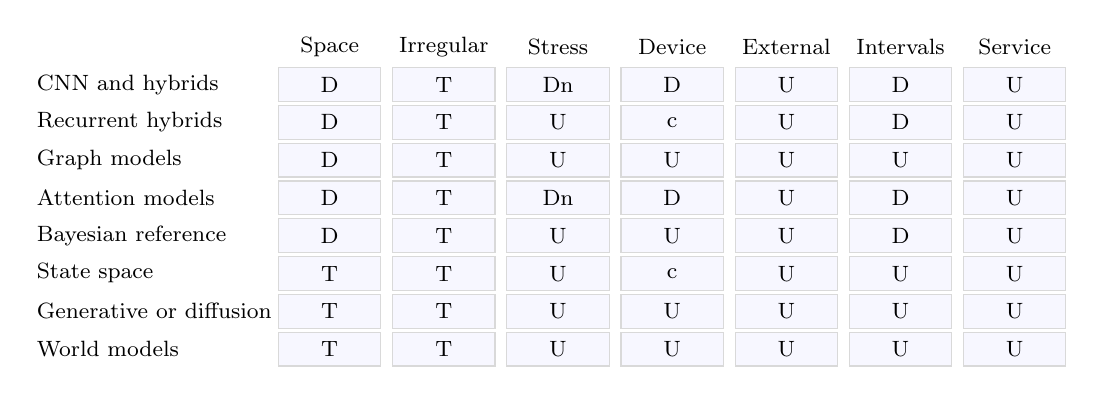
\begin{tikzpicture}[x=1.45cm,y=.48cm,font=\footnotesize]
\foreach \x/\s in {2.6/Space,3.6/Irregular,4.6/Stress,5.6/Device,6.6/External,7.6/Intervals,8.6/Service} {\node[align=center] at (\x,0) {\s};}
\foreach \y/\s in {1/CNN and hybrids,2/Recurrent hybrids,3/Graph models,4/Attention models,5/Bayesian reference,6/State space,7/Generative or diffusion,8/World models} {\node[anchor=west] at (-.05,-\y) {\s};}
\foreach \y/\vals in {1/{D,T,Dn,D,U,D,U},2/{D,T,U,c,U,D,U},3/{D,T,U,U,U,U,U},4/{D,T,Dn,D,U,D,U},5/{D,T,U,U,U,D,U},6/{T,T,U,c,U,U,U},7/{T,T,U,U,U,U,U},8/{T,T,U,U,U,U,U}} {
\foreach \val [count=\j from 0] in \vals {\pgfmathsetmacro{\xx}{2.6+\j}\node[draw=black!15,fill=blue!3,minimum width=1.3cm,minimum height=.43cm] at (\xx,-\y) {\val};}}
\end{tikzpicture}
\caption{Evidence-oriented model comparison. D: demonstrated for the stated property in at least one illustrative study; T: a design capability or extension motivated by method papers, requiring task evaluation; U: not established in the assessed evidence. Dn denotes a limited artificial-noise stress test, not validated robustness to device loss or site shift. c: not established in the 22; a latency or size figure is reported at abstract level by complement records whose device is not stated. Intervals include performance or predictive intervals and do not imply complete calibration. External means an untouched external test; service means an evaluated connected service. Rows overlap: a hybrid counts in every family it contains, and in each hybrid the spatial prior is carried by its convolutional or graph component. Supporting studies for D cells. Space: CNN and hybrids E07, E10, E12, E17, E18, E22; recurrent hybrids E12, E17, E22; graph E06, E14; attention E13; Bayesian E19. Stress: E11, a multi-scale patching encoder coded in both rows. Device (a latency or memory figure on the implied class of device): CNN E01, E05; attention E11. Intervals: CNN E01, E22; recurrent E22; attention E20; Bayesian E19. c: recurrent C1, C2; state space C3. Rows are not prevalence estimates.}
\label{fig:heatmap}\end{figure*}
Four considerations guide the comparison. \emph{Spatial prior}: convolution assumes a regular grid, a graph network assumes a known or learnable topology, and attention assumes neither but pays for it in data. \emph{Irregularity}: CNN--RNN hybrids and plain Transformers assume regular steps unless gaps are encoded, whereas time-aware recurrences and neural ODEs can encode elapsed time explicitly. Discrete state-space models, including a standard Mamba implementation, need appropriate time encoding or discretization when gaps vary. \emph{Missingness}: most families need imputed inputs; generative and diffusion models can impute but add their own error. \emph{Resource cost}: sequence scaling, embedding width, graph density, windowing, precision, and implementation jointly determine cost; dense attention can be quadratic in token count, while volumetric convolution can require substantial activation memory. These are properties by design. Fig.~\ref{fig:heatmap} separates them from what the twenty-two studies demonstrate: explicit spatial modeling is shown by convolutional components, alone or inside the recurrent hybrids that the recurrent row marks, by one attention network over an fMRI grid (E13), by graph models and by the Bayesian reference, and never by a recurrent layer on its own; a resource figure on the implied class of device is shown only for convolutional models (two studies) and an attention-based model (one), and the complement records add abstract-level latency reductions for recurrent and state-space models without naming the device (Section~\ref{sec:iotcomplement}); the assessed set does not establish robustness to operational missingness or an untouched external site, or an end-to-end service evaluation. A controlled artificial-noise test in sMAPEN is narrower evidence~\cite{lin2024smapen}. Intervals on performance and predictions are distinguished from full calibration. Generative, diffusion, state-space, and world models are discussed through method papers and proposed extensions rather than represented by a comparable implementation in the 22-study set.

\subsection{From Acquisition Conditions to Model Choice}
\label{sec:decision}
\begin{table*}[tp]
\centering
\caption{Use-case decision matrix: from acquisition conditions to candidate model families and the verification required before use. Candidate families follow Section~\ref{sec:history}; the last column gives the illustrative studies in each use case. Links and placements are proposed design choices; the retained evidence does not establish all verification requirements for any row.}
\label{tab:decision}
\footnotesize
\setlength{\tabcolsep}{2.5pt}
\renewcommand{\arraystretch}{1.12}
\begin{tabularx}{\textwidth}{|>{\raggedright\arraybackslash}p{2.35cm}|>{\raggedright\arraybackslash}p{1.6cm}|>{\raggedright\arraybackslash}p{1.9cm}|>{\raggedright\arraybackslash}p{2.6cm}|>{\raggedright\arraybackslash}p{2.75cm}|X|>{\raggedright\arraybackslash}p{1.55cm}|}
\hline
Use case & Cadence & Spatial structure & Link and placement & Candidate families & Verification before use & Studies \\
\hline
Glucose forecasting from CGM & 5--15\,min & None & BLE to phone; phone or gateway & Dilated CNN or TCN; time-aware RNN; state space & Subject-disjoint and later-period test with a gap; calibrated prediction intervals; latency on the phone & \cite{Li2020GluNet,Lim2025VirtualCGM} \\
\hline
Movement, gait and eating from body-worn IMUs & 100\,Hz & Body-segment layout (Rel) & BLE; summaries on the device & int8 CNN; graph over segments & Pathological cohort, subject-disjoint; latency and memory measured on the device & \cite{Kyritsis2019EatingBehavior,verbiest2023gaitstride,herath2026parkinson} \\
\hline
Cardiorespiratory signals (ECG, PPG, heart rate) & 1\,Hz--1\,kHz & Channels (MC) & BLE or Wi-Fi; wearable or gateway & CNN--RNN; graph over signal features & Device-standard error limits against an ambulatory reference; held-out cohort & \cite{liu2024cignn,wang2025vo2} \\
\hline
Home ambient and camera sensing & 25--240\,Hz & Sensor array or image grid & Wi-Fi; edge box; images kept local & CNN; 3D-CNN; pose-based networks & Subject-disjoint under home conditions (view, light, bed); latency on the edge box & \cite{liu2025sleepposture,chan2026sitstand,zhu2024ippg} \\
\hline
Neural and cardiac signals moving to portable devices (EEG, MCG, EMG) & 250\,Hz--5\,kHz & Montage or electrode array & Clinic network; edge in the clinic & CNN--GRU; ViT; graph networks & Segment- and repetition-level leakage excluded; cross-site test; latency on the target board & \cite{2,hussein2022seizure,li2026edgeischemia,lin2024smapen} \\
\hline
Imaging sequences (fMRI, CMR, DXA) & Scan or visit & Voxel or anatomical grid & Hospital network; scanner-side or cloud & 3D-CNN; ConvLSTM; spatiotemporal GCN & Patient-level split; held-out center without adaptation & \cite{9,4,5,glaser2022deep} \\
\hline
Longitudinal records & Months & None & Batch EHR exchange (FHIR); cloud, per visit & Longitudinal Transformer; deep joint model; state space & Unadapted external registry; calibration curves at each horizon & \cite{lin2022deep,nitski2021long} \\
\hline
Population surveillance & Monthly or annual & Administrative regions & Batch; cloud & Bayesian spatiotemporal; CNN; STGNN & Temporal hold-out; spatial cross-validation; posterior coverage & \cite{3,XiaoLi2016DiabetesSpatiotemporal} \\
\hline
\multicolumn{7}{@{}>{\raggedright\arraybackslash}p{\dimexpr\textwidth-4\tabcolsep\relax}@{}}{\footnotesize TCN: temporal convolutional network. BLE: Bluetooth Low Energy. EHR: electronic health record; FHIR: Fast Healthcare Interoperability Resources. Other abbreviations as in Tables~\ref{tab:datasets} and~\ref{tab:evidence}.}
\end{tabularx}
\end{table*}
Table~\ref{tab:decision} turns the taxonomy into a selection aid. The first decision is cadence and placement, not architecture: a constrained link or microcontroller may require features to be fixed at the sensing tier, depending on the raw payload and the available budget, while visit-cadence records make sequence length short and per-patient history the main signal. The second is the spatial structure actually present---a sensor layout or anatomical grid justifies a spatial prior; a set of channels without known geometry does not. The third is the verification the use case demands before a model is trusted, whose unit follows the use case: subjects for individual-level transfer, and appropriate time or regional holdouts for population forecasting, with target-device latency and memory for device placement. The final column shows how thin the support is: most rows rest on one to four studies, and the retained evidence does not establish all of the proposed verification conditions for any row.

\subsection{Comparing Costs Under a Common Workload}
\label{sec:workload}
Architectural complexity is informative only once the workload is fixed. With $T$ time steps, $N$ spatial nodes or tokens and $|E|$ graph edges, dense attention over all space--time tokens has interactions proportional to $(NT)^2$, and a factorized spatial-then-temporal layer to $TN^2+NT^2$---not $N^2+T^2$, which omits the number of positions at which each operation runs. Graph aggregation helps when $|E|\ll N^2$, but building or learning a dense adjacency removes that advantage; three-dimensional kernels inflate activation memory; and a recurrent or selective state-space model keeps a bounded state at inference while training may store a long history. Training memory, inference memory, parameter storage and communication payload should therefore be reported separately, and a small parameter count does not guarantee a small peak activation. Sequence length must be read in physical time: 300 samples span five minutes at 1\,Hz but three seconds at 100\,Hz, downsampling can remove the transient that defines the endpoint, and the window itself imposes an acquisition delay that no network can beat.

Matched hardware matters. sMAPEN takes 97.93\,ms on a Raspberry Pi 4B, while the ischemia model takes 4.7\,ms on a desktop CPU~\cite{lin2024smapen,li2026edgeischemia}; the numbers cannot rank the architectures because signals, tasks, windows, devices and implementations all differ, whereas within sMAPEN a faster but less accurate TCN is a meaningful task-specific trade, and the stride study's memory footprint answers yet another question~\cite{verbiest2023gaitstride}. A reproducible resource measurement states hardware, clock or power mode, runtime, precision, batch size, input dimensions, warm-up, and continuous or intermittent execution; reports a latency distribution under load rather than the fastest call; separates flash from peak RAM; and states the energy boundary (processor, sensing board, or gateway with radio). No universal threshold follows from the 22-study set.

\subsection{Model Selection as a Constrained Decision}
\label{sec:constrainedselection}
Table~\ref{tab:decision} first filters candidates by endpoint, decision time, input contract, placement and target population. A proposed constrained comparison is
\begin{equation}
\begin{aligned}
\min_{m,p}\quad &\widehat{\mathcal{L}}_{\mathrm{target}}(m,p)\\
\text{subject to}\quad &L_{95}(m,p)\leq L_{\max},\quad M(m,p)\leq M_{\max},\\
&E(m,p)\leq E_{\max},\quad B(m,p)\leq B_{\max},
\end{aligned}
\label{eq:selectionbudget}
\end{equation}
where $m$ is the model, $p$ its placement, $\widehat{\mathcal L}_{\mathrm{target}}$ the loss under the target validation protocol, $L_{95}$ the 95th-percentile end-to-end latency, $M$ peak working memory, $E$ energy and $B$ transmitted bytes over a stated interval. Budgets are use-case inputs, not clinical thresholds derived here, and feasibility also needs adequate availability and a justified abstention policy. Matched baselines isolate the source of a gain---persistence or autoregression for temporal value, a statistical spatial model or temporal-only ablation for geometry, local-only training for federation---and giving a multimodal model more inputs than its comparator confounds information with architecture. Compressed artifacts must be re-evaluated, since unchanged mean accuracy does not preserve calibration, minority-class performance or robustness~\cite{5,verbiest2023gaitstride}.

\subsection{Joint Predictive and Service Evaluation}
\label{sec:jointservice}
An offline model is evaluated conditional on a complete input window; a connected service must also obtain the window, process it on time and decide whether the result is still valid when delivered. Excluding difficult or delayed windows can make a model look better without informing users better, while a slightly weaker local model may answer during an outage when a remote one cannot. We therefore propose recording every scheduled prediction opportunity. Let $V_i$ indicate that opportunity $i$ produced an output meeting prespecified input-quality, freshness, timing and identity conditions; for $K$ opportunities report
\begin{equation}
\widehat{\rho}=\frac{1}{K}\sum_{i=1}^{K}V_i,\qquad
\widehat{e}_{\mathrm{valid}}=
\frac{\sum_{i=1}^{K}V_i\,\ell_i}{\sum_{i=1}^{K}V_i},
\label{eq:servicecoverage}
\end{equation}
where $\ell_i$ is the task loss. Coverage $\widehat{\rho}$ describes availability under the declared rule, not clinical benefit; $\widehat{e}_{\mathrm{valid}}$ describes accepted outputs, which can differ systematically from the target population, so opportunities without labels stay in the availability denominator. A rejection analysis should separate an absent measurement, an expired observation, a missed deadline, an unsupported input regime and a deliberate abstention, because they call for different remedies and can co-occur---a power outage hits sensor, link and inference together, so marginal availabilities should not simply be multiplied. Time-resolved reports (length of invalid intervals, recovery after disconnection, error against observation age) distinguish a service that misses one long period from one that misses scattered opportunities, and both terms of~\eqref{eq:servicecoverage} should be reported within prespecified subgroups, since camera extraction failures, adherence and gateway access vary across participants. In an offline replay the same timestamped trace, with the same disruptions, can be sent to device, gateway and server configurations, each producing predictions, validity flags and resource measurements for identical opportunities; this links an architectural advantage to deployment conditions but does not replace an external cohort or an impact study.

\subsection{Applying the Decision Framework to Three Workflows}
\label{sec:workedchoices}
The following design analyses apply the framework to conditions illustrated by the reviewed studies; they are not new experiments or treatment recommendations.

\emph{A wearable forecast with intermittent connectivity.} The raw-rate budget of~\eqref{eq:rawrate} decides whether the signal can leave the wearable, and peak memory and energy decide whether inference can stay there. A dilated CNN or small recurrent model suits a short regular window, elapsed-time features become necessary when gaps are part of the served input, and a state-space model is a candidate to benchmark rather than a demonstrated device solution here. GluNet and the virtual-CGM study use different information sets---forecasting from previous glucose versus inferring glucose without current CGM~\cite{Li2020GluNet,Lim2025VirtualCGM}---so a fair placement experiment fixes one regime, replays measured gaps, and records whether a forecast was possible, how old its inputs were and how error changed after reconnection.

\emph{A camera workflow that transmits derived motion.} Converting smartphone video into joint-angle sequences reduces transmission and image retention but changes what the predictor sees: in the sit-to-stand example~\cite{chan2026sitstand}, landmarks in the video do not mean that the downstream temporal convolution encodes skeletal adjacency. A matched-channel ablation tests whether adjacency adds information, a separate experiment tests pose-extraction quality and availability, and latency must include capture, landmark extraction, filtering, prediction and display. Subject-level splits keep a person's trials together, and a home-use claim also needs the intended camera placement, lighting, mobility limits and the rate of failed extractions.

\emph{A visit-cadence model linked to wearable summaries.} Adding weekly wearable summaries to a longitudinal risk model does not make it a synchronized twin. The comparison is clinical history alone versus history plus the stream at the same decision times, retaining device availability, summary age and ownership-related missingness; if the stream exists only for a subgroup, complete-case gains do not transfer to the full population. Serial DXA and registry studies show accumulating-history prediction~\cite{glaser2022deep,lin2022deep,nitski2021long}, not the value of an unmeasured stream, and a linked deployment would still need identity matching, time alignment, freshness, external calibration and a frozen-model external test.

\section{Spatiotemporal Models in Digital Health}
\label{sec:models}
\begin{table*}[tp]
\centering
\caption{Integrated evidence for the twenty-two illustrative studies, grouped by task. Comparator types include matched baselines, ablations, literature values, and reference instruments; they support different inferences. Score pairs are printed at the precision of the source, and each difference is computed from the displayed pair. Values are not comparable across rows. E01--E22: the illustrative set; $^{\dagger}$ten records selected from the PubMed rule-positive pool, the other twelve retained from drafting. C1--C7: IoT-engineering complement from the Xplore-only and IoT-term screen, extracted from abstracts and not counted among the 22.}
\label{tab:evidence}
\footnotesize
\setlength{\tabcolsep}{2.5pt}
\renewcommand{\arraystretch}{1.12}
\begin{tabularx}{\textwidth}{|>{\raggedright\arraybackslash}p{1.7cm}|>{\raggedright\arraybackslash}p{0.4cm}|>{\raggedright\arraybackslash}p{0.7cm}|>{\raggedright\arraybackslash}p{2.25cm}|>{\raggedright\arraybackslash}p{3.1cm}|X|>{\raggedright\arraybackslash}p{0.7cm}|>{\raggedright\arraybackslash}p{0.95cm}|>{\raggedright\arraybackslash}p{1.55cm}|>{\raggedright\arraybackslash}p{0.62cm}|}
\hline
Study & IoT & Sp. & Model & Task; headline result & Reported comparator; difference & Val. & UQ; Sg & Resource & Ref. \\
\hline
\multicolumn{10}{|l|}{\emph{Glycemic forecasting and inference}} \\
\hline
E01 Li & N & T & Dilated CNN (GluNet) & 30-min forecast, OhioT1DM; RMSE 19.28\,mg/dL & ARX 21.54; $-2.26$ & W, A & PI$^{*}$ & Phone, 6\,ms & \cite{Li2020GluNet} \\
\hline
E02 Lim & N & T & BiLSTM $+$ attention & Glucose inference; RMSE 19.49\,mg/dL & Own ablation 19.74; $-0.25$; ablation better at 15--45\,min$^{\ddagger}$ & W & -- & -- & \cite{Lim2025VirtualCGM} \\
\hline
\multicolumn{10}{|l|}{\emph{Detection and estimation from wearable, ambient or camera sensing}} \\
\hline
E03 Kyritsis & N & T & CNN $+$ LSTM & Intake-cycle detection; F1 0.913 & Authors' prior method 0.878; $+0.035$ & S & -- & -- & \cite{Kyritsis2019EatingBehavior} \\
\hline
E04 Liu$^{\dagger}$ & N & MC & Causality-informed STGNN & BP, internal set; MAD 3.20/1.85\,mmHg & GRU 3.97/2.04; $-0.77$/$-0.19$ & S, A & --; Sg & -- & \cite{liu2024cignn} \\
\hline
E05 Verbiest$^{\dagger}$ & N & T & int8 CNN on MCU & Stride length; bias 0.07 $\pm$ 4.3\,cm & None on the same data & S & -- & MCU, 14\,kB RAM & \cite{verbiest2023gaitstride} \\
\hline
E06 Herath$^{\dagger}$ & N & Rel & Pretrained ST graph encoder & PD detection; balanced acc.\ 0.834, AUC 0.842 & XGBoost 0.814, $+0.020$ (n.s.); random forest AUC 0.898, $-0.056^{\ddagger}$ & S & --; Sg & -- & \cite{herath2026parkinson} \\
\hline
E07 Liu$^{\dagger}$ & N & Rel & Parallel CNN, accelerometer array & Sleep posture; acc.\ 98.42\% & ShuffleNetV2 92.16\%; $+6.26$ pts & R & -- & -- & \cite{liu2025sleepposture} \\
\hline
E08 Chan$^{\dagger}$ & N & MC & STS Dynamics Net & Knee OA detection; AUC 0.7759 & FCN 0.7231, $+0.0528$; marker motion capture 0.7855, $-0.0096$ (n.s.)$^{\ddagger}$ & S & --; Sg & -- & \cite{chan2026sitstand} \\
\hline
E09 Wang$^{\dagger}$ & N & MC & CNN--LSTM $+$ attention & Oxygen uptake; $R^2$ 0.9621 & Nearest attention variant 0.9586; $+0.0035$ & S & -- & -- & \cite{wang2025vo2} \\
\hline
E10 Zhu$^{\dagger}$ & N & Anat & CNN $+$ temporal shift & SpO$_2$; MAE 1.10\%, RMSE 1.19\% & MMFM MAE 1.04, $+0.06^{\ddagger}$; RMSE 1.48, $-0.29$ & ? & -- & -- & \cite{zhu2024ippg} \\
\hline
E11 Lin$^{\dagger}$ & N & MC & Multi-scale patching encoder & Hand kinematics; $R^2$ 0.8163 & sBERT 0.6276; $+0.1887$ & R & -- & Pi 4B, 97.93\,ms & \cite{lin2024smapen} \\
\hline
\multicolumn{10}{@{}l@{}}{\footnotesize Codes and abbreviations are defined below the continuation of this table.}\\
\end{tabularx}
\end{table*}

\begin{table*}[tp]
\centering
\addtocounter{table}{-1}
\caption{(Continued) Integrated evidence for the twenty-two illustrative studies and the IoT-engineering complement.}
\footnotesize
\setlength{\tabcolsep}{2.5pt}
\renewcommand{\arraystretch}{1.12}
\begin{tabularx}{\textwidth}{|>{\raggedright\arraybackslash}p{1.7cm}|>{\raggedright\arraybackslash}p{0.4cm}|>{\raggedright\arraybackslash}p{0.7cm}|>{\raggedright\arraybackslash}p{2.25cm}|>{\raggedright\arraybackslash}p{3.1cm}|X|>{\raggedright\arraybackslash}p{0.7cm}|>{\raggedright\arraybackslash}p{0.95cm}|>{\raggedright\arraybackslash}p{1.55cm}|>{\raggedright\arraybackslash}p{0.62cm}|}
\hline
Study & IoT & Sp. & Model & Task; headline result & Reported comparator; difference & Val. & UQ; Sg & Resource & Ref. \\
\hline
\multicolumn{10}{|l|}{\emph{Classification and segmentation from clinical instruments}} \\
\hline
E12 Liu & A & Anat & CNN $+$ GRU brain map & Depression, EEG; acc.\ 89.63\% & L-TCN 86.87\%; $+2.76$ pts & R, A & -- & -- & \cite{2} \\
\hline
E13 Zhang & R & Anat & STANet & Depression, fMRI; acc.\ 82.4\% & Own ablation 79.5\%; $+2.9$ pts & S & -- & -- & \cite{9} \\
\hline
E14 Kong & R & Rel & Spatiotemporal GCN & Depression, fMRI; acc.\ 84.1\% & Comparators in a figure only & S, A & -- & -- & \cite{4} \\
\hline
E15 Hussein$^{\dagger}$ & A & MC & Multi-channel ViT & Seizure prediction, CHB-MIT; sens.\ 99.8\% & Literature 99.7, $+0.1$; Kaggle AES 90.3 vs 94.2, $-3.9^{\ddagger}$ & S, A & -- & -- & \cite{hussein2022seizure} \\
\hline
E16 Li$^{\dagger}$ & A & T & Phase-space CNN fusion & Ischemia screening, MCG; AUC 0.865 & 1D-CNN 0.857, $+0.008$, 2.6$\times$ faster & S & -- & Desktop CPU, 4.7\,ms & \cite{li2026edgeischemia} \\
\hline
E17 Bohoran & R & Anat & Pruned BConvLSTM U-Net & Aortic segmentation, CMR; Dice 0.989 & Unpruned 0.980; $+0.009$ & R & -- & Energy, CO$_2$e & \cite{5} \\
\hline
\multicolumn{10}{|l|}{\emph{Population-level forecasting and mapping}} \\
\hline
E18 Thaipisutikul & R & Adm & Multivariate CNN & National depression counts; MAE 449.7 & SARIMAX 518.4; $-68.7$ & P, A? & -- & -- & \cite{3} \\
\hline
E19 Li & R & Adm & Bayesian spatiotemporal & Diabetes prevalence mapping & Not applicable; estimation only & 0 & CrI & -- & \cite{XiaoLi2016DiabetesSpatiotemporal} \\
\hline
\multicolumn{10}{|l|}{\emph{Longitudinal risk prediction}} \\
\hline
E20 Lin and Luo & R & T & TransformerJM & Dynamic survival; iAUC 0.890/0.812 & MATCH-net 0.895/0.825; $-0.005$/$-0.013^{\ddagger}$ & S, A & Brier, CI & -- & \cite{lin2022deep} \\
\hline
E21 Nitski & R & T & Transformer & 1/5-yr mortality, SRTR; AUROC 0.804/0.733 & Abstract: four deep models vs logistic regression, Transformer best ($p<0.0001$); UHN only after fine-tuning & Abs.; A & 99\% CI & -- & \cite{nitski2021long} \\
\hline
E22 Glaser & R & Anat & DenseNet $+$ RNN & All-cause mortality; AUROC 0.79 & Metadata sequence 0.76; $+0.03$ & S & CI; Sg & -- & \cite{glaser2022deep} \\
\hline
\multicolumn{10}{|l|}{\emph{IoT-engineering complement (abstract-level; outside the 22; Section~\ref{sec:iotcomplement})}} \\
\hline
C1 Bhatti & N & T & CNN--LSTM $+$ attention & Fall phases; F1 0.98 & Prior methods; values n/r & ? & -- & $<$20\,ms; device n/r & \cite{bhatti2025falls} \\
\hline
C2 Trabelsi & A & MC & Distilled CNN--BiGRU & Seizure prediction; acc.\ 97\% & Teacher 99\%; $-2$ pts & ? & -- & Latency $-69$\%; device n/r & \cite{trabelsi2025kdepilepsy} \\
\hline
C3 Kim and Gahm & A & MC & Cross-gated Mamba & EEG decoding; bal.\ acc.\ up to $+6.6$\% & Transformers & ? & -- & Latency $-7.1$\%; device n/r & \cite{kim2026cgmeeg} \\
\hline
C4 Chu & N & T & Spiking network & ECG, MIT-BIH; acc.\ 95.34\% & ADC $+$ ANN; 42.4$\times$ fewer FLOPs & ? & -- & 24.6\,kFLOPs, simulated & \cite{chu2021neuromorphicecg} \\
\hline
C5 Huynh & N & T & ResNet $+$ Transformer & AF, CinC 2017; acc.\ 98.33\% & n/r & ? & -- & 184K parameters & \cite{huynh2026afdetect} \\
\hline
C6 Wang & A & Anat & Factorized 3D CNN & Assay partitions; F1 0.968 & Best frame-based baselines & R & -- & 113\,ms/stack, edge & \cite{wang2026timesight} \\
\hline
C7 Raghuraman & N & T & Event-driven CNN, in-memory chip & Arrhythmia, MIT-BIH; acc.\ 98.61\% & Deep baselines (best) & R & -- & 5\,$\mu$s, 100--150\,$\mu$J, 40\,nm chip & \cite{raghuraman2026cimecg} \\
\hline
\multicolumn{10}{@{}>{\raggedright\arraybackslash}p{\dimexpr\textwidth-4\tabcolsep\relax}@{}}{\footnotesize IoT: N IoT-native, A IoT-adaptable, R record-based (Section~\ref{sec:iotstatus}). Sp.: as in Table~\ref{tab:datasets}. Val.\ (validation level, Section~\ref{sec:quality}): S whole subjects or patients held out \emph{within-cohort} (one cohort, split internally); P later period of a population series; W later period of the same subjects; R record-level split (segment, scan, sample or repetition), so a person can be on both sides; Abs.: assessed from the abstract only, which reports the second registry only after fine-tuning (A), the full protocol not being established; ? unit of split not stated; 0 no hold-out; A a second cohort or site used only after retraining, refitting, fine-tuning, pooling or per-site fitting, which is not an untouched external test (A?: retraining not stated). UQ: PI$^{*}$ predictive bounds with coverage not assessed; CI confidence or bootstrap interval on performance; CrI posterior credible interval; Brier: integrated Brier score, not by itself a calibration measure; no assessable study shows a calibration curve; the 99\% CI of the abstract-only record is on AUROC and does not establish calibration. n/r: not reported. Sg: results by demographic or clinical subgroup. $^{\ddagger}$Unfavorable to the proposed model on that comparison. Difference: proposed minus comparator (pts: percentage points). CNN, (Bi)LSTM, GRU, GCN, ViT: convolutional network, (bidirectional) long short-term memory, gated recurrent unit, graph convolutional network, vision Transformer; STGNN, ST graph: spatiotemporal graph neural network; MCU: microcontroller; ARX, SARIMAX: autoregressive models with exogenous inputs; FCN, L-TCN: fully convolutional and temporal convolutional networks; MMFM, sBERT, STANet, STS: authors' model names. RMSE, MAE, MAD: root mean squared, mean absolute and mean absolute difference errors; (i)AUC, AUROC: (integrated) area under the receiver operating characteristic curve; acc.: accuracy; sens.: sensitivity; n.s.: not significant as reported. BP: blood pressure; PD: Parkinson's disease; OA: osteoarthritis; AF: atrial fibrillation; ADC: analog-to-digital converter; ANN: artificial neural network; FLOPs: floating-point operations; BiGRU: bidirectional GRU; Mamba: selective state-space model; MIT-BIH, CinC 2017: public electrocardiogram benchmarks; SpO$_2$: oxygen saturation; CO$_2$e: carbon-dioxide equivalent; others as in Table~\ref{tab:datasets}.}
\end{tabularx}
\end{table*}
This section reviews implemented systems, with the illustrative comparison anchored in the primary studies of Table~\ref{tab:evidence}. Studies are grouped by task. Numbers are interpreted within each paper, distinguishing matched baselines from ablations, instrument references, and published values obtained under potentially different protocols; ``n/r'' (not reported) and unfavorable results are kept apart, since an unreported comparison is missing evidence while an unfavorable one is evidence. The studies were published between 2016 and 2026 and span dietary, diabetes, depression and cardiac work together with the wearable, ambient and camera-based studies sampled from the rule-eligible pool. Two patterns cut across the groups. First, the unit of analysis is not uniform within a domain: diabetes and depression each contain individual-level sensing studies and population-level surveillance studies, which should not be pooled. Second, deployment characteristics are almost never reported. Eleven of the twenty-two draw on data captured by a body-worn, ambient or consumer device. We keep what each study \emph{reports} about cost and where inference runs separate from the placement \emph{we} infer: the resource column of Table~\ref{tab:evidence} is reported, while the placements of Fig.~\ref{fig:taxonomy} and Table~\ref{tab:decision} are our reading and not evidence of deployment. Of the twenty-two, five state anything about model cost or latency~\cite{5,Li2020GluNet,verbiest2023gaitstride,lin2024smapen,li2026edgeischemia}, with three reporting a figure on the class of device the work implies---a phone, a microcontroller or a portable board---although the microcontroller figure for latency is a toolchain estimate and only its memory footprint was measured~\cite{Li2020GluNet,verbiest2023gaitstride,lin2024smapen}. None reports sustained data rate, bandwidth, connectivity assumptions or an update strategy, and none evaluates a deployed end-to-end connected service; we do not generalize beyond the set, whose provenance we state.

\subsection{Validation Levels and Leakage}
\label{sec:quality}
We grade validation in five levels rather than as a yes--no field. Twelve assessable studies hold out whole subjects or patients within a cohort; the abstract-only Nitski record is retained separately, one holds out a later period of a population series~\cite{3}, and two hold out a later period of the same subjects for personalized glucose models~\cite{Li2020GluNet,Lim2025VirtualCGM}. Four split at the level of a record---a one-second EEG segment~\cite{2}, a scan of a patient who contributes several~\cite{5}, a sensor sample~\cite{liu2025sleepposture} or a movement repetition~\cite{lin2024smapen}---so the same person can appear on both sides; one does not state the unit of its split~\cite{zhu2024ippg}; and one estimates on the full sample with no hold-out at all~\cite{XiaoLi2016DiabetesSpatiotemporal}. Among the seven additional-cohort evaluations assessed in detail, six involve retraining, refitting, fine-tuning, pooling, or separate site-specific fitting~\cite{2,4,Li2020GluNet,lin2022deep,liu2024cignn,hussein2022seizure}; adaptation is unclear in the population-transfer example~\cite{3}. The abstract of the Nitski record reports its second registry only after fine-tuning, which is also adaptation, while its full protocol is not established; an untouched external test is not established by the retained extraction, and, specifically for personalized glucose prediction, an additional held-out-subject experiment reported by the authors, in which a generalized glucose model loses accuracy against personalized ones (root mean squared error 24.9 against 20.6\,mg/dL)~\cite{Li2020GluNet}. Two further leakage risks are specific to the pipeline: resampling or normalizing before the split, and building a graph from all participants before cross-validation, which one blood-pressure study does not exclude~\cite{liu2024cignn}.

\subsection{Within-Study Comparisons by Task}
\label{sec:withinstudy}
\emph{Glycemic forecasting.} GluNet~\cite{Li2020GluNet} forecasts glucose 30 and 60 minutes ahead with a dilated CNN and a personalized model per subject, beating the best of four published predictors on every dataset (with lower RMSE on OhioT1DM at 30 minutes), and reports 6\,ms per prediction on an Android phone. Lim et al.~\cite{Lim2025VirtualCGM} infer glucose from app-entered diet, exercise and weight in 171 healthy adults with a bidirectional LSTM and dual attention, splitting each subject's days in time with a one-day gap against leakage; they compare only ablations, one of which beats the full model at 15--45 minutes, and the authors note that models given previous glucose are clearly superior at short horizons. Patient-specific management of this kind is increasingly framed as a predictive digital twin~\cite{Faruqui2024}.

\emph{Wearable, ambient and camera sensing.} The subject-disjoint studies report small margins. A pretrained spatiotemporal graph encoder for Parkinson's disease leads six classical baselines by 0.020 in balanced accuracy, not significantly, and trails random forest by 0.056 in area under the receiver operating characteristic curve (AUC)~\cite{herath2026parkinson}; smartphone sit-to-stand dynamics detect symptomatic knee osteoarthritis 0.0528 AUC above FCN (0.7759 versus 0.7231) but 0.0096 below marker-based motion capture~\cite{chan2026sitstand}; an attention-enhanced CNN--LSTM improves oxygen-uptake $R^2$ by 0.0035 over its nearest attention variant (0.9621 versus 0.9586)~\cite{wang2025vo2}; and a causality-informed STGNN lowers cuffless blood-pressure error by 0.77\,mmHg systolic against a GRU~\cite{liu2024cignn}. Dietary data appear as wearable inertial series or image sequences of eating, modeled by CNN--LSTM, 3D-CNN or ConvLSTM networks~\cite{Rouast2020IntakeGesture}; the dietary study here detects in-meal intake cycles from a smartwatch 0.035 F1 above the authors' earlier method, leave-one-subject-out over twelve subjects and twenty-one staged meals~\cite{Kyritsis2019EatingBehavior}; its endpoint is intake-cycle behavior rather than food composition, so it does not establish which nutrients were consumed or whether an intervention changes health. The int8 stride-length network reports agreement with an optical reference but no comparator on the same data~\cite{verbiest2023gaitstride}. The largest margins in the set come from record-level splits: a smart-bed accelerometer array classifies sleep posture 6.26 percentage points above the best published network on a sample-level split~\cite{liu2025sleepposture}, and an electromyography encoder raises $R^2$ by 0.19 over its best comparator while testing on held-back repetitions of the same subjects' movements~\cite{lin2024smapen}. Face-video oxygen saturation is better than its best comparator on root mean squared error but worse on mean absolute error, on a split whose unit is not stated~\cite{zhu2024ippg}.

\emph{Clinical instruments.} EEG depression classification gains 2.76 points over a temporal convolutional network, on segments rather than subjects~\cite{2}; an fMRI aggregation network gains 2.9 points over its best ablation at the subject level~\cite{9}; and a spatiotemporal GCN that also predicts two-week treatment response reports its comparators only in a figure, run separately within each of two sites~\cite{4}. A multi-channel vision Transformer for seizure prediction matches the best published sensitivity on scalp EEG under leave-one-subject-out validation but trails it by 3.9 points on an intracranial benchmark, comparing against literature values rather than re-run baselines~\cite{hussein2022seizure}. Magnetocardiography ischemia screening gains 0.008 AUC over a one-dimensional CNN whose confidence interval overlaps and which runs 2.6 times faster~\cite{li2026edgeischemia}; the reported 4.7\,ms latency was measured on a desktop central processing unit (CPU), not on the edge board the work targets. A pruned ConvLSTM U-Net segments the aortic lumen 0.009 Dice above its unpruned form and reports energy and carbon-equivalent cost, with scans rather than patients split~\cite{5}. Center-to-center protocol variation and real-time demands remain the obstacles the cardiac literature names~\cite{6}.

\emph{Population and longitudinal prediction.} A multivariate CNN forecasts national monthly depression counts with mean absolute error 69 below a seasonal autoregressive model, on seventy monthly points~\cite{3}; a Bayesian spatiotemporal model maps county diabetes prevalence with posterior intervals and no predictive hold-out~\cite{XiaoLi2016DiabetesSpatiotemporal}. Among the longitudinal studies, TransformerJM trails the MATCH-net comparator on integrated AUC in both cohorts while having the lowest integrated Brier score~\cite{lin2022deep}; sequence models over serial dual-energy X-ray absorptiometry (DXA) gain 0.03 AUC over a metadata sequence model~\cite{glaser2022deep}; and, by its abstract, a Transformer outperforms three other deep models and logistic regression for liver-transplant mortality (AUROC 0.804 at one year, 99\% CI 0.795--0.854), with the second registry evaluated only after fine-tuning; the interval describes discrimination, not calibration, and the full protocol is not verified here~\cite{nitski2021long}.

\subsection{Uncertainty, Calibration and Subgroups}
Discrimination, calibration, uncertainty and subgroup performance are separate properties, and the set reports them unevenly. No study shows a calibration curve or calibration slope for a risk it displays. One reports an integrated Brier score~\cite{lin2022deep}, a useful measure of prediction error that mixes discrimination and calibration and does not by itself establish calibration. The assessable records include posterior intervals~\cite{XiaoLi2016DiabetesSpatiotemporal}, confidence or bootstrap intervals on performance~\cite{lin2022deep,glaser2022deep}, and predictive 95\% bounds with coverage not established~\cite{Li2020GluNet}; the abstract-only record gives 99\% intervals on AUROC~\cite{nitski2021long}. None of these intervals is evidence of calibration. Subgroup analyses are described in four full-text-assessed studies~\cite{glaser2022deep,liu2024cignn,herath2026parkinson,chan2026sitstand}; detailed subgroup coverage for the abstract-only Nitski record is not assessed here. Code availability is recorded in audit file A06 but does not itself establish a reproducible pipeline. Prospective clinical impact is not established by the illustrative set.

\subsection{Cross-Domain Patterns}
\label{sec:patterns}
\paragraph{Small samples, high dimensions} Imaging data are high dimensional but small in sample~\cite{4,5,6}, and many wearable cohorts enroll fifteen to thirty participants~\cite{verbiest2023gaitstride,liu2025sleepposture,wang2025vo2}, which risks overfitting and poor transfer; physical priors, self-supervised pretraining~\cite{herath2026parkinson} and federated training are the proposed remedies, but none is evaluated for transfer here. Read together with the validation levels, the within-study margins suggest a design lesson: in this set, margins measured on subject-disjoint splits are task-specific, sometimes small and sometimes unfavorable, while the largest---6.26 points of accuracy and 0.19 in $R^2$---coincide with record-level splits, so a reported margin should be read through its split before it informs model choice.

\paragraph{Multimodal fusion} Fusing environmental, behavioral and clinical data with the primary signal yields richer assessments---socioeconomic covariates for prevalence maps~\cite{XiaoLi2016DiabetesSpatiotemporal}, ECG with photoplethysmography for blood pressure~\cite{liu2024cignn}---and statistical models encode physical transport through Bayesian hierarchies~\cite{liu2022convectionDiffusion}; Section~\ref{sec:DT} states when fusion fails.

\paragraph{Deployment and efficiency} Pruning~\cite{5} and int8 quantization~\cite{verbiest2023gaitstride} are the two compression techniques actually evaluated, and only the second was run on the target device; one study shows that a simpler model reaches a similar AUC at a third of the latency~\cite{li2026edgeischemia}, the trade an edge deployment most needs reported.

\paragraph{Explainability} These studies mostly supply attention maps~\cite{2,4}, but attention is not explanation: Jain and Wallace~\cite{jain2019attention} showed that attention distributions can often be replaced without changing the prediction, Serrano and Smith~\cite{serrano2019attention} that the highest-weighted components are often not those whose removal changes the output, and Wiegreffe and Pinter~\cite{wiegreffe2019attention}, defending a weaker reading, agree that attention alone does not establish faithfulness. Clinicians ask for actionable justification rather than saliency~\cite{tonekaboni2019clinicians}, and high-stakes decisions may favor inherently interpretable models~\cite{rudin2019stopexplaining}.

\subsection{Longitudinal Evidence within the Taxonomy}
\label{sec:longitudinal}
Three studies in Table~\ref{tab:evidence} (E20--E22) use longitudinal clinical records or serial clinical imaging. We include them because the twin argument of Sections~\ref{sec:DT} and~\ref{sec:world_model_dt} rests on synchronization, and they are the clearest evidence in the set that re-prediction from accumulating history is feasible, although one trails its strongest comparator~\cite{lin2022deep}. All sample history a few times a year at clinical encounters; a visit-token Transformer could accept wearable-derived weekly summaries beside laboratory panels, so a connected deployment changes the sampling regime rather than the model class, and serial DXA, scans years apart, is not a health-IoT modality. Whether between-visit wearable summaries add information over the clinical trajectory none of the three addresses.

\subsection{Matching Validation to the Deployment Claim}
\label{sec:validationclaim}
\label{sec:effectinterpretation}
A split defines the population to which a result can transfer. A within-person later-period test supports a known person's future under the observed regime, and a subject-disjoint test new people within the sampled cohort; neither establishes transfer to a new device, hospital, region or home, and time or regional holdouts can be the right unit for population forecasts. An external test freezes preprocessing, graph construction, weights, thresholds and calibration before touching the new institution; fine-tuning, pooling, per-site fitting or threshold selection on its labels makes an adaptation experiment, which answers a different question. Personalization needs chronological discipline---what measurements and labels exist at enrollment and at each update---and retrospective cleaning must not supply information unavailable at the historical decision time.

A numerical gain is interpretable only relative to its outcome, comparator, information set and protocol. A gain over a weaker ablation does not establish superiority over every named model; county mapping supplies statistical context and stride agreement a measurement comparison, not an architectural gain. Difference calculations must respect reporting precision. Table~\ref{tab:evidence} therefore prints each score pair at the precision of its source and computes the difference from that pair: GluNet's 19.28 against 21.54\,mg/dL gives $-2.26$, and the smart-bed accuracy of 98.42\% against 92.16\% gives $+6.26$ points; rounding both values first would have given $-2.2$ and $+6.2$. Absolute percentage-point changes differ from relative percentages, and small differences need uncertainty at the correct sampling unit---repeated windows from one person are not independent patients, and overlapping intervals do not settle a paired comparison. The synthesis therefore offers task-specific comparisons rather than a pooled ranking or a universal benefit from adding spatial structure.

\section{Spatiotemporal Models in Medical Digital Twins}
\label{sec:DT}
This section labels its two evidence states: the twin systems it cites are implemented, while the requirements, checklists and failure conditions it states are our proposals.

\subsection{Digital Twins in Digital Health}
We use digital twin for a patient-specific virtual state with a declared synchronization process and an accountable feedback path. General cyber-physical frameworks motivate describing the physical and computational boundaries~\cite{NIST2021}; clinical verification and validation must be established separately for the intended function~\cite{Sel2025VVUQ}. Early work formalized the healthcare twin as a virtual patient built from biological and omics data, promising precision medicine while raising ethical questions~\cite{Bruynseels2018DigitalTwins}. Faruqui \emph{et al.}\ paired a transfer-learned network with a clinician-guided controller to generate daily lifestyle recommendations for type 2 diabetes~\cite{Faruqui2024}. Among the twin work cited here, an example with independent predictive validation is mechanistic rather than learned: Silfvergren \emph{et al.}\ fit organ crosstalk and hepatic fluxes to several clinical studies, predicted an independent study correctly and personalized the response to an individual~\cite{Silfvergren2022}---an explicitly offline twin with no return path from a sensed patient. A 2026 physics-informed twin of cerebral hemodynamics goes further toward patient specificity: it assimilates physiological knowledge and patient data, was tested on in vivo experiments and simulated data, and, personalized to six neurocritical-care patients, forecast cerebral blood flow more accurately than machine-learning models~\cite{briggs2026cerebral}. It is a hybrid mechanistic--data-assimilation example with retrospective personalization in a very small cohort, not evidence of prospective clinical benefit or of a synchronized feedback service. Closed-loop wearable bioelectronics, reviewed the same year, couple sensing, AI-based control and therapy on the body~\cite{gao2026closedloop}; such a loop acts on a patient, but closing a control loop neither requires nor establishes a patient-specific twin or an action-conditioned world model, and that review itself makes clinical value conditional on stable interfaces, transparent safety mechanisms and evidence of patient benefit.

\subsection{Operational Requirements}
\label{sec:twinreq}
``Twin'' is used loosely, so we state six requirements a system must meet, each with what would demonstrate it. \emph{Patient specificity}: the state is bound to one identified individual, with identity resolved across that person's devices and records; assessed using patient-specific error where repeated observations permit it, together with appropriate population and subgroup calibration. \emph{Synchronization}: the state is updated from new observations at a stated cadence and latency, with each update versioned and a freshness indicator on the output; demonstrated by error as a function of time since the last update. \emph{Fusion}: sources at different rates are aligned on one time base with their provenance; demonstrated by performance with each source withheld at its real availability rate. \emph{Updating}: what is re-estimated at each synchronization---state only, or parameters---and how drift is detected; demonstrated by performance under device and population shift. \emph{Feedback}: a path from the virtual to the physical side, with the person responsible for each action named; demonstrated by the decision changes it causes. \emph{Validation}: evidence at the level of Fig.~\ref{fig:maturity} appropriate to the use, from external validation for a displayed risk to prospective evaluation for a recommended action. By these requirements the longitudinal studies of Section~\ref{sec:longitudinal} meet patient specificity and partial updating at visit cadence, the illustrative set does not establish synchronization with a sensed stream under a declared freshness contract, and an end-to-end feedback pathway or untouched external validation is not established for the illustrative set.

\subsection{Data Collection, Fusion and Its Limits}
Data collection is the hardest stage of building a medical twin, because sources differ in sparsity and rate---sparse electronic health record (EHR) entries, second-level intensive-care monitoring, interval imaging---so alignment is a prerequisite, and cross-modal fusion the usual answer to the gaps of any single modality~\cite{baltrusaitis2019multimodal}. Fusion is not monotonically beneficial: an added modality brings noise at low signal-to-noise, bias when availability differs across subgroups (a twin fusing a wearable inherits the demographics of who wears it), cost in devices, bandwidth and alignment, and a new failure point, since a fused model is only as available as its least reliable input unless trained for modality dropout. Patient heterogeneity compounds this: identical indicators can imply different risks across populations~\cite{obermeyer2016predicting}. Post-hoc attribution reports what the model weighted, not whether to act, so a twin needs a person adjudicating identity, device provenance and implausible values at intake, approving re-synchronizations that shift a risk stratum, reading every output that changes therapy, and auditing subgroup calibration, with routing to a human whenever uncertainty is high, the input regime has changed or the patient lies outside the training cohort.

\subsection{Communication Options and Interoperability}
\label{sec:protocols}
Communication options must be compared within their own layer: radio rates, latency targets and application delivery semantics are not interchangeable, and none is a measured end-to-end service figure. FHIR and IEEE 11073 support exchange and device profiles, but calibration, identity, unit equivalence, provenance and event-time alignment still need application checks.

\paragraph{Bearers} Bluetooth Low Energy (BLE) reached about 0.24\,Mb/s of application throughput in the configuration measured in~\cite{gomez2012ble}; its delay depends on the connection interval, its range is short, and a low duty cycle supports long battery life, so a wearable's sampling rate and usable throughput must be budgeted separately. Wi-Fi (IEEE 802.11) offers nominal tens to hundreds of Mb/s shared within a cell, with millisecond delays plus contention over tens of meters, and can carry images or model updates at a higher energy cost; coverage gaps and gateway availability must be measured, not assumed. Cellular 4G and 5G provide megabits to gigabits per second over a wide area~\cite{li20185giot}; the 1\,ms 5G figure is a radio target, not an end-to-end delay, and energy use and subscription cost constrain placement and update cadence even when a device can avoid a nearby gateway. LoRaWAN sits at the other extreme, with about 0.3 to 50\,kb/s, delays of seconds set by the duty cycle, kilometer range and years on a primary cell~\cite{raza2017lpwan}: it suits small, infrequent payloads, while a large model update may take too long for the intended cadence.

\paragraph{Application protocols} Message Queuing Telemetry Transport (MQTT) runs over the transmission control protocol (TCP) with a few bytes of overhead per message~\cite{mqtt5standard}; its delay follows the link plus broker queueing, its persistent session costs energy on a sleeping device, and its quality-of-service levels govern delivery semantics, not physiological completeness or a clinical deadline---recovery after a gap needs suitable session behavior, queueing or an explicit buffer. The Constrained Application Protocol (CoAP) runs over the user datagram protocol (UDP) with a compact header for constrained nodes~\cite{rfc7252}; confirmable messages add retransmission, and observation needs a separate extension. Neither protocol has a universal energy advantage, and interoperability standards sit above these choices without substituting for them.

\paragraph{Payload and update budgets} Before choosing placement, estimate raw rate as
\begin{equation}
R_{\mathrm{raw}}=C f_s b,
\label{eq:rawrate}
\end{equation}
where $C$ is channel count, $f_s$ sample rate, and $b$ bits per sample. Six channels at 100 Hz and 16 bits require 9600 bits/s, or 1200 bytes/s and about 103.7 MB/day using decimal units, before headers, encryption, retries, or storage overhead. A hypothetical one-million-parameter int8 artifact contains about 1 MB; at effective 10 kb/s throughput its transfer takes at least 800 seconds. These are arithmetic design examples, not results extracted from a trial. Summaries reduce payload but may remove information needed for future reprocessing; caching and delta updates require measurement. An edge-intelligent AIoT twin architecture makes the same trade explicit: for simulated fall and instability monitoring with a 100\,Hz inertial node per patient, it sends event-driven state updates of about a hundred bytes instead of a continuous raw stream (about 104\,MB per day), and reports orders-of-magnitude lower simulated device energy and bandwidth than continuous cloud and edge baselines~\cite{jun2026aiottwin}. The costs are computational-simulation results; hardware validation, real sensor traces, detection errors and clinical deployment remain future work, so the design is evidence about a payload budget, not about a synchronized patient service.

\paragraph{Freshness and recovery} End-to-end delay includes window acquisition, preprocessing, buffering, transmission, queueing, inference, and presentation; overlapping stages should not be blindly added. Observation age is
\begin{equation}
A(t)=t-u(t),
\label{eq:freshness}
\end{equation}
where $u(t)$ is acquisition time of the newest valid observation available at decision time $t$. Fast inference on a delayed batch can have low processor latency and high $A(t)$. Report both with missed deadlines and valid-output coverage. During outages, explicitly choose local inference, buffering, or a stale-state fallback. Sequence IDs, timestamps, and deduplication are needed on reconnection; reconciliation must not overwrite the historical information state. The illustrative set does not establish this complete communication contract.

\subsection{Privacy and Federated Learning}
\label{sec:fl}
\begin{figure}[tp]
\centering
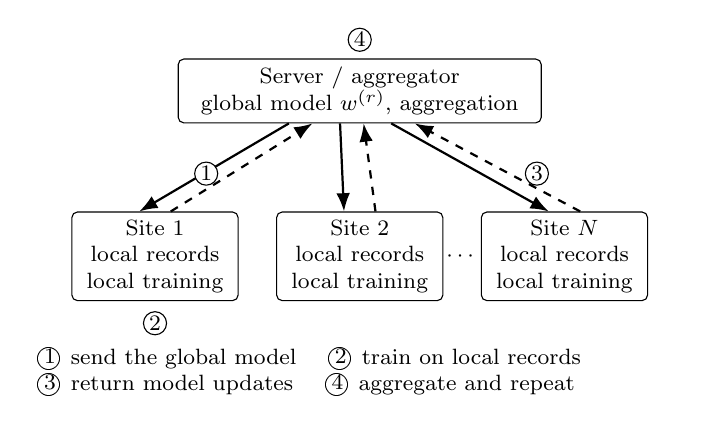
\begin{tikzpicture}[font=\footnotesize, >=Latex,
  box/.style={draw, rounded corners=2pt, align=center, inner sep=3pt},
  stp/.style={circle, draw, inner sep=0.6pt, font=\footnotesize, fill=white}]
\node[box, text width=44mm] (srv) at (0,0) {Server / aggregator\\global model $w^{(r)}$, aggregation};
\node[box, text width=19mm] (s1) at (-2.6,-2.1) {Site 1\\local records\\local training};
\node[box, text width=19mm] (s2) at (0,-2.1) {Site 2\\local records\\local training};
\node[box, text width=19mm] (sn) at (2.6,-2.1) {Site $N$\\local records\\local training};
\node at (1.3,-2.1) {$\cdots$};
\foreach \s/\dx in {s1/-0.9, s2/-0.25, sn/0.4} {
  \draw[->, thick] ([xshift=\dx cm]srv.south) -- ([xshift=-2mm]\s.north);
  \draw[->, thick, dashed] ([xshift=2mm]\s.north) -- ([xshift=\dx cm + 3mm]srv.south);}
\node[stp] at (-1.95,-1.05) {1};
\node[stp] at (-2.6,-2.1) [yshift=-8.5mm] {2};
\node[stp] at (2.25,-1.05) {3};
\node[stp] at (0,0) [yshift=6.5mm] {4};
\node[align=left, anchor=north, text width=82mm] at (0,-3.15) {\textcircled{\footnotesize 1} send the global model \quad \textcircled{\footnotesize 2} train on local records\\ \textcircled{\footnotesize 3} return model updates \quad \textcircled{\footnotesize 4} aggregate and repeat};
\end{tikzpicture}
\caption{The federated learning cycle. Solid arrows: the global model sent to each site; dashed arrows: model updates returned for aggregation. Raw records stay at the site. Transport encryption, secure aggregation, and differential privacy address different threats and require separate implementation.}
\label{fig:flcycle}
\end{figure}
Healthcare data are a frequent target of fraud and ransomware~\cite{Seh2020HealthcareDataBreaches}, and centralized storage is especially exposed, motivating training without moving raw data~\cite{rieke2020digitalhealth}. Federated learning sends model updates rather than raw data; transport encryption, secure aggregation, and differential privacy must be implemented separately~\cite{aouedi2022FLmedical}. In the usual cycle (Fig.~\ref{fig:flcycle}) a global model is sent to participating sites, each trains it on its own records, and the returned updates---plain unless secure aggregation or encryption is added---are aggregated over many rounds. It costs communication, suffers when site data are not independent and identically distributed (non-IID), and remains open to adversarial exposure; on its own it supplies neither encryption nor a privacy guarantee. Inside a twin, the proposed design has local twins on edge or hospital servers refine a shared spatiotemporal network and send updates to an aggregator~\cite{aouedi2022FLmedical,nguyen2022FLsmarthealthcare}; quantitative evidence for such designs remains preliminary. A federated spatiotemporal twin should report at minimum client availability and participation, non-IID heterogeneity including site and device shift, rounds to convergence, update size and total bandwidth, round latency, client energy, compute and memory ceilings, straggler and dropout handling, personalization back to each site, the attacks of Section~\ref{sec:attack} evaluated, the differential-privacy budget with its accuracy cost, and comparison with centralized and local-only baselines.

\subsection{Synchronizing State Without Silently Changing the Model}
\label{sec:synchronization}
\label{sec:federatedstate}
A state update incorporates new observations with a fixed model; a parameter update changes the mapping applied to future observations. The two must be logged separately: fast repeated prediction does not establish retraining, and new weights do not establish a fresh patient state. Each output should be bound to patient identity, acquisition times, preprocessing, model version, state version and unresolved quality flags, and when a delayed laboratory result or corrected packet arrives, reconciliation may improve the current estimate but must preserve the state that informed the earlier decision. Cadence follows the endpoint---a visit-level risk need not refresh at sensor rate, while a displayed continuous estimate needs an expiry or fallback rule---and error and availability should be evaluated against time since the last valid input, because a refreshing dashboard is not evidence of fresh physiology. Patient-specific history is not a patient-specific parameter or an identified treatment response, and a few observations from one person do not establish calibration for that person. Feedback needs a named recipient, a permitted response, a validity interval and an audit trail; a reviewed decision and an autonomous actuator carry different requirements.

Federated rounds and local state updates run on different clocks. New global weights should not silently reinterpret an existing state: record the global version, local adaptation, migration rule and state version so that a prediction stays reproducible after rollback. Communication should be measured separately at training and inference boundaries (update bytes alone omit rounds, participation, retries and model distribution), centralized, local-only and federated models compared on one endpoint with their accessible data stated, and per-site results reported, since a cross-site mean can hide harm at one site.

\subsection{Visualization: Rendering Is Not Synchronization}
Twins enable personalized visualization: extended-reality overlays have been used for surgical guidance and planning~\cite{Auvinet2018AR}, and virtual brain models used in doctor--patient communication raised satisfaction about 25\% above the average of a standardized patient-experience survey across 257 patients~\cite{Louis2021VR}. Such rendering is judged on comprehension, which is evidence about the interface, not the model behind it. An interface bound to a continuously updated patient state should be judged on calibration of the displayed risk and on whether the clinician's decision changes and improves outcome; we are not aware of a study evaluating a synchronized health twin interface against clinical endpoints.

\section{World-Model-Based Digital Twins in Digital Health}
\label{sec:world_model_dt}
This section is a \emph{proposed framework and research agenda}, not a synthesis of evaluated systems: within the illustrative evidence considered here we did not establish a health twin that learns an action-conditioned latent transition and has been validated against patient outcomes. The move from twins to world models has so far been articulated for mobile edge intelligence rather than clinical care~\cite{Zheng2026DTtoWM}, which is not evidence of clinical use.

\subsection{Distinguishing the Adjacent Concepts}
Two criteria separate the adjacent concepts; without them a survey renames latent trajectory prediction as a world model and repeated prediction as a twin. For the planning question considered here, an \emph{action-conditioned world model} supplies a learned transition that can be rolled forward under specified actions. A controlled state-space model can have the same mathematical form; the labels are not mutually exclusive. A mechanistic simulator instead specifies some or all transition structure from domain theory. A system is a \emph{digital twin} only when it is bound to one identified individual and kept synchronized with a path back to that individual; one-way updating is a digital shadow, and repeated prediction alone does not establish the synchronization and feedback claims of a twin. The working distinctions below state which components each concept assumes and the evidence behind each claimed function. Readiness must be assessed for an implemented system and intended use, rather than assigned to a whole model class.

\paragraph{Working distinctions} We describe each concept by seven components: an observation encoder, a latent state, a transition model, an action or intervention model, a decoder or reward or outcome head, a policy or planner, and synchronization to a specific physical instance. These are components of a working template, not universal architectural requirements, and the categories overlap: a controlled state-space model may also be a world model. A \emph{state-space or disease-progression model} centers on a latent state propagated between observations by a transition; control inputs and planning may be present but are not assumed. A \emph{generative model} centers on its decoder: it models the data distribution and can sample from it, but carries no notion of intervention. A \emph{mechanistic simulator} specifies its transition from domain theory rather than learning it, so its parameters are physically meaningful. A \emph{causal model} centers on the intervention component and answers interventional and counterfactual queries under stated identification assumptions. An \emph{action-conditioned world model} couples a transition with an action model, giving a learned, action-conditioned transition that can be rolled forward without the real system. \emph{Model-based reinforcement learning} uses a learned or specified model with an objective and a planner or policy; the transition need not be learned. A \emph{digital shadow} is defined by automatic one-way flow from the physical instance to the virtual one, with no feedback to the physical side, whereas a \emph{digital twin} is bound to one specific instance and kept synchronized, with feedback returning to that instance. Synchronization with accountable feedback, rather than a particular neural architecture, therefore distinguishes the intended twin function.

\paragraph{Evidence scope} The evidence behind these concepts differs within the material considered here, and this scope neither describes the maturity of a whole model class nor certifies deployment readiness. State-space, generative, and model-based reinforcement-learning models enter only as method context; the mechanistic simulator appears through a retrospective example; causal models were not systematically assessed; action-conditioned health world models now have retrospective implementations (Section~\ref{sec:recentwm}) but no outcome-validated or synchronized one; the digital shadow is an operational definition; and for the digital twin only partial components are cited.

\subsection{Implemented Medical World Models, 2026}
\label{sec:recentwm}

Seven 2026 sources were assessed at this revision, and they separate cleanly by what they establish. Three are implemented models carrying retrospective or simulated evidence only: EHRWorld~\cite{mu2026ehrworld}, ChronoMedicalWorld~\cite{wang2026chronomedicalworld} and the cerebral hemodynamics twin~\cite{briggs2026cerebral}. One is a framework whose cost figures come from simulation alone, the edge AIoT twin~\cite{jun2026aiottwin}. Three are frameworks or reviews that implement nothing and measure nothing: the closed-loop wearables review~\cite{gao2026closedloop}, the medical world-model review~\cite{chen2026medicalwm} and the imaging world-model verification framework~\cite{wimalasiri2026verifiable}, all three also compared as reviews in Table~\ref{tab:related-surveys}. None of the seven establishes a synchronized clinical service or prospective patient benefit. Two action-conditioned medical world models have now been implemented and evaluated retrospectively; both are arXiv preprints, outside the two databases searched, and neither enters the twenty-two. EHRWorld fine-tunes language models on 110{,}513 MIMIC-IV hospitalization episodes so that inquiry events return observations and intervention events update an implicit patient state, and on 579 held-out episodes it outscores general-purpose language models on simulated inquiry results and retains more accuracy over successive rounds~\cite{mu2026ehrworld}. ChronoMedicalWorld encodes structured interventions together with patient--coach messages into a recurrent latent transition over 2{,}232 patients of a kidney-care platform and, on a patient-level test split, lowers rollout error by about 7\% against a prompted language-model baseline~\cite{wang2026chronomedicalworld}. Both show that action semantics and rollout stability can be engineered and measured, which earlier versions of this section could only propose. Neither identifies treatment response: the actions are the ones recorded under routine care, so the models forecast trajectories under the historical policy, and ChronoMedicalWorld states that it does not adjust for confounding. Neither has external or prospective evaluation, a sensed IoT stream, or a synchronized feedback path to a patient.

Two contemporaneous syntheses sharpen what an evaluation must show. A verification framework for imaging world models separates simulation fidelity, roll-out stability and clinical plausibility, defines an effective planning horizon as the last step before a stated loss quantile exceeds a clinical tolerance under the observed action policy, and finds that none of nine audited imaging models reports such a horizon, a counterfactual-consistency check or a clinically meaningful subgroup analysis~\cite{wimalasiri2026verifiable}; because that horizon is estimated on-policy, it does not certify off-policy plans. A review of 98 medical world-model sources finds most retrospective, task-specific or preclinical and lists inconsistent action semantics, limited causal identifiability and long-horizon error accumulation as the main barriers~\cite{chen2026medicalwm}. Our framework is consistent with both and differs in where it starts: from the acquisition contract, the link and the inference placement that decide what state such a model can observe, how fresh it is, and whether a connected service can act on it.

\subsection{Prediction, Simulation and Causal Identification}
\label{sec:causal}
Four tasks are often run together. \emph{Prediction} estimates what will be observed next under the care actually given. \emph{Simulation} rolls a learned transition forward under a chosen action sequence. \emph{Counterfactual identification} asks whether that rollout equals what would have happened under the action, which requires assumptions the data cannot supply: no unmeasured confounding of action and outcome, positivity (every action of interest observed in comparable patients), and a correct model of how actions act. \emph{Decision support} then ranks actions for a clinician and adds safety and accountability requirements of its own. An action argument in $P_\phi$ makes simulation possible; it does not make the simulated effect causal. Clinical actions are chosen because of the patient's state---confounding by indication---so a transition trained on observational histories learns how treated patients evolved, not what treatment did; actions outside the historical policy are extrapolation, whose evaluation requires estimator-specific assumptions, a known or adequately estimated historical policy where needed, and sufficient action overlap. Until these are addressed, through target-trial emulation~\cite{hernan2016targettrial}, randomized or quasi-experimental data, or hybrid mechanistic--learned transitions whose action pathway is specified, a health world model is a simulator of plausible trajectories, not an estimator of intervention effects, and any ranking it produces needs human review and prospective safety evaluation before it informs care.

\subsection{Specifying the Intervention Question and Rollout Uncertainty}
\label{sec:interventionquestion}
\label{sec:rolloutuncertainty}
Before a rollout, specify the eligible population, decision time, candidate strategies, follow-up horizon, outcome and comparator, with time zero aligning eligibility, strategy assignment and follow-up; information recorded after assignment must not enter the baseline state, and a strategy such as lifestyle advice needs enough content, intensity and timing to be reproducible. Prediction under the recorded policy differs from the outcome under an intervention strategy: observational identification needs consistency, exchangeability given the recorded history, positivity and an appropriate estimator, and treatment-dependent confounding is not removed by adjusting for every observed variable in one regression. Target-trial emulation makes the question and assumptions explicit~\cite{hernan2016targettrial} but does not by itself remove unmeasured confounding or inadequate overlap, so action support should be reported where the model will be queried---long action sequences can be unsupported even when every single action appears somewhere---and unsupported queries rejected.

Verification checks that pipelines preserve temporal order, action labels map to real interventions, constraints prevent impossible states and rollouts are reproducible under missing, delayed or shifted inputs. Validation cannot rest on held-out histories alone, because most interventions are counterfactual: it needs calibration across horizons, subgroup analysis, external cohorts, action coverage and prospective study~\cite{Sel2025VVUQ}. Rollout uncertainty comes from the starting state, measurement error, parameters, model structure and future actions; sampling trajectories from one fitted model captures only the uncertainty that model represents, intervals should be checked for coverage across horizons, groups and degraded input regimes, and a usable system separates aleatoric from epistemic uncertainty and abstains when no reliable recommendation is possible. For planning, test whether plausible changes in initialization, calibration or action coding reverse the ranking of strategies; an on-policy effective planning horizon~\cite{wimalasiri2026verifiable} is a useful stability summary but does not certify off-policy plans, and a safety filter tested against declared constraints establishes behavior in those tests only. Independent intervention evidence, then prospective silent-mode and impact evaluation, remain separate gates before a simulated ranking informs care.

\subsection{Attack Surface of a World-Model-Based Twin}
\label{sec:attack}
Active simulation widens the attack surface: a compromised predictive twin produces a wrong number, a world-model twin a wrong plan, and an actuating loop a wrong action. Four attacks are specific to the action-conditioned setting: \emph{sensor spoofing} drives the latent state that seeds every rollout; \emph{action-label tampering} inverts an intervention's estimated effect while predictive accuracy stays intact; \emph{state poisoning} through malicious federated updates shifts the learned dynamics; and \emph{planner manipulation} makes an unsafe trajectory look optimal. The layers of Fig.~\ref{fig:taxonomy} add the rest, across confidentiality, integrity, availability, privacy and safety.

At the device, link and edge, stored samples can be read from a lost wearable, sensors spoofed and firmware tampered to shift calibration, batteries exhausted and links jammed, encrypted traffic still analyzed for behavior, and a cached model or buffered windows extracted from a gateway; a microcontroller can be driven to its resource or thermal limits, and an on-device model is open to membership inference and unsafe out-of-distribution inference~\cite{saha2022mcuml}. Per-device authentication and key storage, signed firmware with calibration provenance and IEEE 11073 profiles~\cite{ieee11073std}, mutually authenticated transport with replay protection and sequence checks, store-and-forward with acknowledgement so that loss is visible, secure boot, signed and reversible model updates, and refusal to infer outside the validated input range belong at these layers.

On the platform and in federated training, record stores are frequent breach targets~\cite{Seh2020HealthcareDataBreaches}; schema or unit drift and label corruption threaten integrity, linkage can expose a subgroup, gradient inversion can recover samples, update poisoning can shift dynamics, stragglers stall rounds, and non-IID clients can yield a model unsafe for a minority site~\cite{nguyen2022FLsmarthealthcare,aouedi2022FLmedical}. Access control with audit, schema validation with FHIR as the contract~\cite{ayaz2021fhir}, provenance for every derived variable, secure aggregation and transport encryption (which federation does not supply), anomaly screening of client updates, a stated differential-privacy budget with its accuracy cost, and per-site evaluation are the corresponding protections. For the twin and planner, a tampered synchronization path makes the twin track a wrong state, lost synchronization leaves a stale twin in service, released rollouts can leak private information, and a manipulated planner yields a wrong action rather than a wrong number~\cite{maes2026leworldmodel}; reviewed identity resolution, versioned state with a freshness indicator, calibration monitoring, an audit log binding outputs to model versions~\cite{Sel2025VVUQ}, evaluated disclosure control, and accountable human review before any clinical action address them. Attacks should be tested by detected and missed events, decision changes, refusals and recovery on replayed data or a disabled-actuation testbed. This is a proposed threat analysis; none of the reviewed studies evaluates these controls for a health world-model twin.

\subsection{Evidence Stages from Prediction to Prospective Use}
\label{sec:maturity}
\begin{figure*}[t]\centering
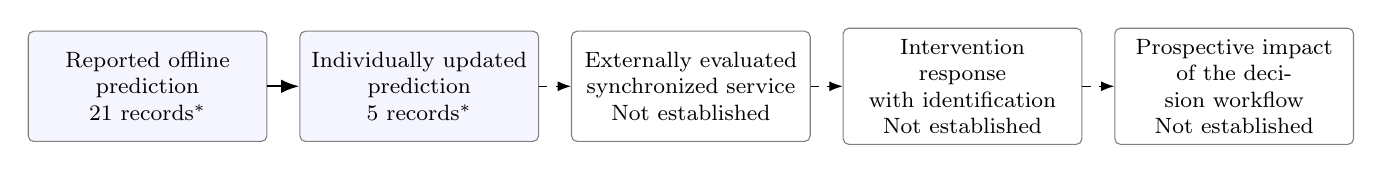
\begin{tikzpicture}[>=Latex,font=\footnotesize,
b/.style={draw=black!50,rounded corners=2pt,align=center,text width=2.75cm,minimum height=1.4cm,inner sep=4pt}]
\node[b,fill=blue!4] (a) at (0,0) {Reported offline\\prediction\\21 records$^{*}$};
\node[b,fill=blue!4] (b) at (3.45,0) {Individually updated\\prediction\\5 records$^{*}$};
\node[b] (c) at (6.9,0) {Externally evaluated\\synchronized service\\Not established};
\node[b] (d) at (10.35,0) {Intervention response\\with identification\\Not established};
\node[b] (e) at (13.8,0) {Prospective impact\\of the decision workflow\\Not established};
\draw[->,thick] (a)--(b);\draw[->,dashed] (b)--(c);\draw[->,dashed] (c)--(d);\draw[->,dashed] (d)--(e);
\end{tikzpicture}
\caption{Proposed evidence stages for increasingly strong intended-use claims. Counts refer only to the illustrative set; $^{*}$includes one abstract-only record. Dashed transitions identify additional evidence requirements, not a universal chronology or a prohibition on earlier simulation research. The later claims are not established by this synthesis.}
\label{fig:maturity}\end{figure*}
Fig.~\ref{fig:maturity} places the reviewed evidence on five stages. Offline prediction is reached by twenty-one of the twenty-two records at the level of a reported predictive endpoint, including one abstract-only record and individually updated prediction by five---three at visit cadence~\cite{lin2022deep,nitski2021long,glaser2022deep} and two per-subject glucose models~\cite{Li2020GluNet,Lim2025VirtualCGM}. No study reaches an externally validated, synchronized twin, and the set does not establish identified intervention responses or prospective impact of a connected decision workflow. The stages distinguish intended-use claims; research can explore simulation before deployment validation, provided its status is clear.

\section{Future Prospects: Spatiotemporal Digital Twins}
\label{sec:future}

Section~\ref{sec:future} turns the observed gaps into measurable technical questions and orders them by what they unblock. All empirical counts refer to the illustrative records assessed here and inherit the purposive selection of Section~\ref{sec:selection}. The illustrative set does not supply a complete evaluation of the sensor-to-twin-to-decision pipeline and its system quantities. \emph{Priority 1} questions can be answered now with existing data and testbeds and gate everything else: benchmarking one task across device, gateway and server placement with latency and energy beside accuracy (G1); re-evaluating reported gains under subject-disjoint and unadapted external splits with a fixed harmonization pipeline (G7); and measuring fusion at realistic modality availability (G2). \emph{Priority 2} questions need multi-site or clinical collaboration: federated training with its system costs reported (G4), faithfulness testing of explanations (G3) and the added value of lifestyle streams (G6). \emph{Priority 3} questions presuppose the first two: an outcome evaluation of a world-model twin (G5) and red-team evaluation of an acting twin (G8).

\emph{Networking directions.} The agenda assumes a communication layer that this literature leaves unspecified, although the bearer and protocol fix the achievable sampling rate, the tolerable loss and whether an update can be pushed (Section~\ref{sec:protocols}). Three questions are concrete enough to attack now: \emph{protocol fit}, including how a selected stack carries versioned model updates and provenance alongside measurements; \emph{a resource budget from model to deployment}, reporting bytes per patient-day at the sensor and after on-device summarization, model bytes per federated round, latency at each placement and energy at each hop as one chain; and \emph{shared testbeds}---needed, for example, to measure on hardware the energy and bandwidth savings that event-driven twin updates have so far shown only in simulation~\cite{jun2026aiottwin}---combining instrumented participants, an edge tier with controllable bandwidth, latency and loss, and a federated coordinator, with released traces so that a reported edge deployment can be replicated.

\begin{table*}[tp]
\centering
\caption{Prioritized research agenda derived from the observed gaps G1--G8. Priority 1 questions can be answered with existing data and testbeds and gate the rest; priority 3 presupposes priorities 1 and 2.}
\label{tab:agenda-a}
\footnotesize
\setlength{\tabcolsep}{2.5pt}
\renewcommand{\arraystretch}{1.12}
\begin{tabularx}{\textwidth}{|>{\raggedright\arraybackslash}p{0.55cm}|>{\raggedright\arraybackslash}p{3.6cm}|>{\raggedright\arraybackslash}p{3.7cm}|X|>{\raggedright\arraybackslash}p{3.6cm}|}
\hline
Pr. & Observed gap & Measurable question & Design and baselines & Metric and success criterion \\
\hline
1 & G1 Sparse cost evidence in this set: five records report some cost figure, three on the implied device class; no measured data rate or bandwidth established & Which families meet the accuracy target inside the memory, energy and bandwidth envelope of a wearable--gateway tier? & One task benchmarked at device, gateway and server placement on a physical testbed; baselines: server model, compressed on-device model, classical predictor & p95 latency, energy per inference, peak memory, bytes per patient-day; non-inferior to the server model at a stated budget \\
\hline
1 & G7 Gains read without their split: the largest margins come from record-level splits; no untouched external site & Do reported gains survive subject-disjoint and unadapted external validation under a fixed harmonization pipeline? & Re-evaluation of published models on public datasets with one harmonization choice varied at a time; baseline: the original split & Change in the headline metric with confidence intervals; variance explained by split and harmonization choices \\
\hline
1 & G2 Incremental fusion value at real modality availability is not established in this synthesis & Does each modality help at its real availability and failure rate? & Leave-one-modality-out and simulated dropout at measured device failure rates; baselines: best single modality, complete-case fusion & Change per modality with confidence intervals and calibration; retain a modality only if it helps at its availability \\
\hline
2 & G4 End-to-end federated system budgets are not established by the illustrative prediction set & What round, bandwidth and energy budget makes federated spatiotemporal training viable across sites with device shift? & Multi-site testbed with measured non-IID split and injected dropout; baselines: centralized, local-only, federated averaging & Rounds to target, bytes per round, client energy, privacy budget with its accuracy cost; better than local-only within site bandwidth \\
\hline
2 & G3 Attention weights alone do not establish explanatory faithfulness & Are attended space--time regions responsible for the prediction? & Perturbation of attended regions; baselines: matched random regions, an interpretable model & Comprehensiveness and sufficiency; attended regions change the output more than random regions \\
\hline
2 & G6 Lifestyle evidence measures behavior, not outcomes & Do wearable lifestyle streams add information beyond the clinical trajectory? & Cohort with paired clinical and lifestyle streams; baseline: clinical-only longitudinal model & Incremental discrimination and calibration across device-ownership strata; interval excludes zero \\
\hline
3 & G5 No outcome-validated action-conditioned synchronized twin established in the assessed set & Does an action-conditioned model rank interventions consistently with trial evidence once confounding is addressed? & Target-trial emulation, then prospective silent-mode use; baselines: model without actions, mechanistic simulator, standard care & Agreement with trial-derived effects; calibration across horizons; uncertainty coverage \\
\hline
3 & G8 Safety of an acting health twin is not established by this synthesis & How much spoofing or action-label corruption changes the plan a twin issues? & Red-team evaluation of a testbed twin under a declared threat model; baseline: undefended twin & Attack success against perturbation budget; detected and missed violations, abstention, decision changes, recovery time; zero observed failures is not proof of zero risk \\
\hline
\multicolumn{5}{@{}>{\raggedright\arraybackslash}p{\dimexpr\textwidth-4\tabcolsep\relax}@{}}{\footnotesize Pr.: priority. p95: 95th percentile. Non-IID: not independent and identically distributed.}
\end{tabularx}
\end{table*}

\subsection{A Reproducible Evaluation Package and the Order of Work}
\label{sec:evalpackage}
A reproducible package links a data manifest (sources, units, acquisition and arrival times, missingness), a split manifest (participants, sites, periods, exclusions) and fitted preprocessing artifacts to the evaluated weights, precision, runtime and input contract, and a measurement trace connects each prediction to those versions with latency, memory, energy, bytes, freshness and valid-output coverage; twins add state and reconciliation logs, and planners action-support, uncertainty, constraint and reviewer logs. Replication differs from re-evaluation: a changed split or pipeline can test transportability without reproducing the original result, so the original score should be preserved and deviations documented, and failure to reconstruct a protocol is not proof that a model is ineffective.

Table~\ref{tab:agenda-a} links each gap to an experiment, comparator and measurable output. First test which predictive gains survive patient-, time- or region-appropriate splits, frozen preprocessing and realistic input availability; then whether deployment, added modalities or cross-site collaboration improve the specified service within its measured budget; intervention ranking additionally needs an identified estimand, action support and independent response evidence. These are research dependencies, not a ban on earlier simulation: gate the claim rather than the architecture.

\section{Review Limitations}
\label{sec:limitations}
\emph{Selection was purposive, not systematic.} Twelve of the studies in Table~\ref{tab:evidence} were assembled while drafting rather than sampled, and the two logged searches put the rule-eligible literature at 593 records against the 22 we synthesize, so no statement about completeness or prevalence follows from any number we report. We did not pre-register a protocol, and one author screened and extracted; the measured error of the screening rule bounds, but does not remove, that limitation.

\emph{IEEE Xplore and IoT-specific coverage.} The ten sampled studies were drawn from the PubMed pool. The 230 Xplore-only records and the 307 IoT-term additions were screened only by textual rules and an AI-assisted abstract assessment, and the seven retained complement records are extracted from abstracts, so engineering work that reports system figures only in its full text, or names its device only there, can be missed. The health-term block itself misses device-centric work (adding IoT terms grows the PubMed arm by 26\%). Both biases run toward clinical and record-based studies and away from IoT-native systems that report latency, energy or bandwidth, so the scarcity of system measurements in Table~\ref{tab:evidence} describes this set and may overstate their absence from the wider literature.

\emph{Search constraints.} Registries, regulatory submissions, unpublished industrial deployments and non-English work are excluded, as is statistical spatiotemporal work before 2015.

\emph{Currency.} The databases were re-searched through 22 October 2026 (Section~\ref{sec:searchupdate}), but arXiv was not a searched source; the 2026 world-model and twin sources of Section~\ref{sec:recentwm} were added from a targeted update, are assessed from their abstracts or accessible text, and do not enter the twenty-two. This literature is moving faster than any snapshot.

\emph{Preprints, publication bias and heterogeneity.} Part of the world model literature exists only as preprints and the published record over-represents positive results, which may make reported performance optimistic relative to less selected deployment populations; the studies differ in cohort, outcome, horizon and split, so we compare numbers only within a study and do not pool or rank them. One study could be verified only from its abstract.

\emph{Judgment in coding.} Spatial structure, IoT status, validation level, family assignment and the demonstrated--design-motivated--not-established marks of Fig.~\ref{fig:heatmap} required judgment, and a different reviewer could code some studies differently; our treatment of deployment characterizes what is reported in the illustrative set rather than measuring the systems, and we did not re-implement any model.

\section{Conclusion}
\label{sec:conclusion}
\emph{RQ1.} The sensing tier fixes data type, sampling cadence and feasible inference placement together, so model selection should start there (Fig.~\ref{fig:taxonomy}, Table~\ref{tab:decision}). Within the illustrative set, ten of the twenty-two studies model it, none uses geographic coordinates, and seven are temporal only.

\emph{RQ2.} Read within each study, the evidence for spatiotemporal deep learning is modest. Under subject-disjoint validation the margins over the best in-study comparator are small and sometimes unfavorable; the largest margins come from record-level splits; an untouched external test is not established in the assessable study protocols; no study shows a calibration curve; and only three report a resource figure on the class of device the work implies. A reported gain should be gated by its split level, an unadapted external test and measured on-device cost before it informs model choice.

\emph{RQ3.} A twin needs patient specificity, synchronization, fusion, updating, feedback and validation (Section~\ref{sec:twinreq}). The illustrative set reaches individually updated prediction at visit cadence; the illustrative prediction set does not establish a fully evaluated sensor-synchronized feedback service.

\emph{RQ4.} A world-model twin is distinguished by an action-conditioned transition and by synchronization with a return path to the individual, and the illustrative evidence does not establish a system meeting both conditions evaluated against patient outcomes. An action-conditioned model simulates; it does not identify intervention effects. Until confounding, action coverage and prospective safety are addressed, Section~\ref{sec:world_model_dt} remains a conceptual framework, and the prioritized agenda of Section~\ref{sec:future} states what would move it forward.

\section*{Acknowledgment}
This work was supported in part by the National Institutes of Health under Grants R56DK114514-01 and R01DK129432 (PI: Fang), and by the National Science Foundation under Award 2428595 (PI: Wang). The content is solely the responsibility of the authors and does not necessarily represent the official views of the National Institutes of Health or the National Science Foundation.

The authors disclose that Anthropic Claude was used for language editing throughout; for restructuring this version, including an earlier reorganization of dataset, quality and deployment tables and drafting text; for drawing Figs.~\ref{fig:taxonomy}, \ref{fig:foundation_arch}, \ref{fig:heatmap} and~\ref{fig:maturity}; and for assisted retrieval of comparator values. OpenAI Codex assisted the final revision, including prose, table restructuring and restoration, source checks, numerical consistency review, and the code-generated framework and evidence figures. In the last revision Anthropic Claude assisted with the scripts for the IoT-complement screen and the 22 October search update, with checking comparator values against the sources, with consolidating the text, and with redrawing Figs.~\ref{fig:taxonomy} and~\ref{fig:fivecat}. The authors retain responsibility for literature selection, source verification, technical interpretation, and the final manuscript.

\IEEEtriggeratref{99}
\bibliographystyle{IEEEtran}
\bibliography{newST}

\end{document}
